% =========================================================
%  Reporte: El Problema del Transporte — Equipo 5
%  Maestría en Ciencia de Datos, INFOTEC
%  Asignatura: Matemáticas 2026-1
%  Mayo de 2025
%
%  Compilar con:
%      pdflatex reporte.tex
%      pdflatex reporte.tex   (segunda pasada para referencias)
% =========================================================

\documentclass[10pt,letterpaper,twocolumn]{article}

% --- Codificación e idioma ---
\usepackage[utf8]{inputenc}
\usepackage[T1]{fontenc}
\usepackage[spanish,es-tabla,es-noindentfirst]{babel}
\usepackage{mathptmx}    % Tipografía Times Roman estilo IEEE
\usepackage[scaled=0.92]{helvet}  % Helvetica para sans-serif

% --- Geometría tipo IEEE ---
\usepackage[letterpaper,
            top=0.75in, bottom=0.85in,
            left=0.65in, right=0.65in,
            columnsep=0.28in,
            footskip=0.4in]{geometry}

% --- Matemáticas ---
\usepackage{amsmath,amssymb,amsfonts}

% --- Gráficos y colores ---
\usepackage{graphicx}
\usepackage{xcolor}
\definecolor{infotec}{HTML}{4A0E2C}
\definecolor{infotecLight}{HTML}{F7F0F3}
\definecolor{azul}{HTML}{1E40AF}
\definecolor{verde}{HTML}{065F46}
\definecolor{grisFondo}{HTML}{F5F5F5}
\definecolor{rojoOscuro}{HTML}{7F1D1D}
\definecolor{terminalBg}{HTML}{1E1E1E}
\definecolor{terminalFg}{HTML}{D4D4D4}
\definecolor{ambar}{HTML}{F59E0B}

% --- Tablas con estilo profesional ---
\usepackage{array}
\usepackage{booktabs}
\usepackage{tabularx}
\usepackage{colortbl}
\renewcommand{\arraystretch}{1.15}

% --- Encabezados de sección estilo IEEE ---
\usepackage{titlesec}
\titleformat{\section}
  {\normalfont\fontsize{11pt}{13pt}\bfseries\color{infotec}\MakeUppercase}
  {\thesection.}{0.5em}{}
\titleformat{\subsection}
  {\normalfont\fontsize{10pt}{12pt}\bfseries}
  {\thesubsection.}{0.4em}{}
\titleformat{\subsubsection}
  {\normalfont\fontsize{9.5pt}{11pt}\bfseries\itshape}
  {\thesubsubsection.}{0.4em}{}
\titlespacing*{\section}{0pt}{1.2ex plus 0.4ex}{0.5ex}
\titlespacing*{\subsection}{0pt}{0.9ex plus 0.3ex}{0.4ex}
\titlespacing*{\subsubsection}{0pt}{0.7ex plus 0.2ex}{0.3ex}

% --- Captions más compactos ---
\usepackage[font=small,labelfont=bf,labelsep=period,
            justification=raggedright,singlelinecheck=false]{caption}
\captionsetup[table]{position=top}
\captionsetup[figure]{position=bottom}

% --- Listings (código Python con resaltado simple) ---
\usepackage{listings}
\lstdefinestyle{pythonStyle}{
  basicstyle=\ttfamily\fontsize{7.5pt}{9pt}\selectfont,
  backgroundcolor=\color{grisFondo},
  frame=leftline,
  framerule=0.8pt,
  rulecolor=\color{infotec},
  framesep=4pt,
  xleftmargin=8pt,
  breaklines=true,
  breakatwhitespace=false,
  showstringspaces=false,
  language=Python,
  keywordstyle=\color{azul}\bfseries,
  commentstyle=\color{verde}\itshape,
  stringstyle=\color{rojoOscuro},
  numbers=none,
  aboveskip=4pt, belowskip=4pt,
  upquote=true,
  literate={á}{{\'a}}1 {é}{{\'e}}1 {í}{{\'i}}1 {ó}{{\'o}}1
           {ú}{{\'u}}1 {ñ}{{\~n}}1 {Á}{{\'A}}1 {É}{{\'E}}1
           {Í}{{\'I}}1 {Ó}{{\'O}}1 {Ú}{{\'U}}1 {Ñ}{{\~N}}1
           {¿}{{?`}}1 {¡}{{!`}}1
}
\lstdefinestyle{terminalStyle}{
  basicstyle=\ttfamily\fontsize{7.5pt}{9pt}\selectfont\color{terminalFg},
  backgroundcolor=\color{terminalBg},
  frame=leftline,
  framerule=0.8pt,
  rulecolor=\color{verde},
  framesep=4pt,
  xleftmargin=8pt,
  breaklines=true,
  showstringspaces=false,
  numbers=none,
  aboveskip=4pt, belowskip=4pt,
  literate={á}{{\'a}}1 {é}{{\'e}}1 {í}{{\'i}}1 {ó}{{\'o}}1
           {ú}{{\'u}}1 {ñ}{{\~n}}1
}
\lstset{style=pythonStyle, columns=fullflexible, keepspaces=true}

% --- Hipervínculos (sin colorear, estilo IEEE) ---
\usepackage[hidelinks,breaklinks=true]{hyperref}

% --- Listas personalizables ---
\usepackage{enumitem}

% --- Inclusión de PDFs externos (para anexo del notebook) ---
\usepackage{pdfpages}

% --- Mejor justificación y separación ---
\usepackage{microtype}
\setlength{\parskip}{0.3ex}
\setlength{\parindent}{1em}

% --- Permitir figuras anchas (column-span: all) ---
\usepackage{stfloats}

% --- Footnote en página de portada ---
\usepackage{titling}

% --- Cabeceras de página ---
\usepackage{fancyhdr}
\pagestyle{fancy}
\fancyhf{}
\renewcommand{\headrulewidth}{0pt}
\fancyfoot[C]{\thepage\ /\ \pageref{LastPage}}
\usepackage{lastpage}

% =========================================================
%  CONTENIDO
% =========================================================
\begin{document}

% ----------- PORTADA -----------
\begin{titlepage}
\thispagestyle{empty}
\begin{center}

\vspace*{0.4in}


\includegraphics[width=1.4in]{img/infotec_bg.png}

\vspace{0.25in}
{\sffamily\bfseries\color{infotec}\Large
Centro de Investigación e Innovación\\en Tecnologías de la Información y\\Comunicación --- INFOTEC\par}

\vspace{0.05in}
{\sffamily\large Maestría en Ciencia de Datos\par}

\vspace{0.5in}
{\sffamily\bfseries\fontsize{20pt}{24pt}\selectfont
El Problema del Transporte:\\
Formulación Primal--Dual,\\
Representación en Grafos\\
y Aplicaciones\par}

\vspace{0.15in}
{\sffamily\itshape\large Reporte de Investigación --- Tema 5: El Problema del Transporte\par}

\vspace{0.5in}

\begin{tabular}{rl}
\textbf{\color{infotec}Asignatura:} & Matemáticas 2026-1 \\
\textbf{\color{infotec}Imparte:} & Dra.\ Briceyda B.\ Delgado \\
\textbf{\color{infotec}Equipo:} & 5 \\
\textbf{\color{infotec}Actividad:} & 4A --- Reporte de Investigación \\
\end{tabular}

\vspace{0.4in}

\begin{minipage}{4.5in}
\centering
\rule{\textwidth}{1.5pt}\\[0.1in]
{\sffamily\bfseries\color{infotec}\large Integrantes\par}
\vspace{0.08in}
{\sffamily\large
Andrés Rangel\\
Santiago Mendoza\\
David Rodríguez\\
Bryan Rodríguez\par}
\vspace{0.1in}
\rule{\textwidth}{1.5pt}
\end{minipage}

\vspace{0.5in}
{\sffamily Ciudad de México --- 2 de mayo de 2026\par}

\end{center}
\end{titlepage}

% ----------- TÍTULO Y RESUMEN (UNA COLUMNA) -----------
\twocolumn[
  \begin{@twocolumnfalse}
    \begin{center}
    {\sffamily\bfseries\fontsize{16pt}{19pt}\selectfont
    El Problema del Transporte: Formulación Primal--Dual,\\Representación en Grafos y Aplicaciones\par}

    \vspace{0.06in}
    {\sffamily A. Rangel, S. Mendoza, D. Rodríguez, B. Rodríguez\par}
    {\sffamily\itshape\small Maestría en Ciencia de Datos --- INFOTEC, México\par}
    \vspace{0.04in}
    \rule{\textwidth}{0.5pt}
    \end{center}

    \vspace{0.1in}
    \noindent\colorbox{grisFondo}{%
    \begin{minipage}{0.97\textwidth}
    \small
    \textbf{Resumen---}
    El Problema del Transporte es uno de los modelos más estudiados de la programación lineal y constituye, junto con su problema dual asociado, un puente natural entre la optimización matemática, la teoría de grafos y la economía de redes. En este reporte se presenta el modelo desde tres ángulos complementarios: (i) la formulación primal del transportista, orientada a minimizar el costo total de distribución sujeto a restricciones de oferta y demanda; (ii) la formulación dual del embarcador, que introduce los precios sombra como herramienta de valoración marginal de los recursos; y (iii) la representación topológica como un grafo bipartito dirigido, donde cada variable de decisión equivale a una arista. Se desarrollan dos ejemplos numéricos resueltos con la biblioteca PuLP de Python: un caso de logística de última milla en e-commerce con datos balanceados, y una distribución de agua en emergencia con restricciones complejas (rutas bloqueadas, capacidades máximas y prioridades obligatorias). El reporte cierra con un análisis comparativo de aplicaciones reales en logística, energía, distribución de emergencia y movilidad urbana, así como con las limitaciones operativas del modelo.
    \end{minipage}}

    \vspace{0.06in}
    \noindent\small\textbf{Palabras clave---} Programación lineal, problema del transporte, dualidad, precios sombra, grafos bipartitos, PuLP, optimización combinatoria, cadena de suministro.

    \vspace{0.15in}
  \end{@twocolumnfalse}
]

% ============================================================
%  1. INTRODUCCIÓN
% ============================================================
\section{Introducción}

El Problema del Transporte es uno de los modelos clásicos de la programación lineal y, en términos de aplicaciones reales, probablemente el más utilizado. En su forma básica, busca determinar la manera más económica de distribuir un producto homogéneo desde varios puntos de origen donde existe oferta hacia varios puntos de destino donde existe demanda, conocidos los costos unitarios de transporte para cada par origen-destino~[1].

El estudio de este modelo es relevante en investigación de operaciones y gestión logística por al menos cinco motivos clave. Primero, su objetivo natural ---minimizar el costo total de distribución--- afecta directamente el desempeño económico de cualquier empresa que mueva mercancías o recursos. Segundo, aunque su nombre sugiere envíos físicos, su estructura matemática se aplica a problemas que no involucran transporte alguno: programación de la producción donde los periodos actúan como fuentes y destinos, programación de mantenimiento de herramientas, asignación de turnos, y muchos otros casos en los que se requiere mover «algo» (incluso intangible) desde donde sobra hacia donde falta~[2].

Tercero, el problema admite algoritmos especializados ---como el método de la esquina noroeste, el método del costo mínimo, el método de aproximación de Vogel y el método de los multiplicadores--- que son sustancialmente más eficientes que el simplex general para esta estructura particular. Cuarto, el modelo es uno de los pilares de la cadena de suministro moderna: gestionar el flujo de bienes, dinero e información entre proveedores, fabricantes y consumidores requiere un equilibrio constante entre capacidad de respuesta y eficiencia, y el problema del transporte es la herramienta básica para encontrar ese equilibrio. Quinto, su representación visual mediante redes (nodos y arcos) y mediante el tablero de transporte facilita la comunicación entre analistas y tomadores de decisiones~[2].

Adicionalmente, el problema admite una \emph{interpretación dual} sumamente útil. La teoría de la dualidad en programación lineal establece que todo programa lineal ---el primal--- tiene asociado otro programa lineal ---el dual---, y que ambos comparten el mismo valor óptimo. En el caso del transporte, mientras el primal representa al transportista que minimiza costos, el dual representa al embarcador que compra producto en los orígenes y lo vende en los destinos buscando maximizar el margen~[3]. Las variables del dual, conocidas como \textbf{precios sombra}, miden el cambio marginal del costo óptimo ante variaciones unitarias en la oferta o la demanda, y son la base teórica del método de los multiplicadores que prueba la optimalidad de una solución~[2].

El presente reporte sigue una estructura clara: la Sección~2 ofrece un estado del arte que recorre los hitos históricos del problema desde Monge hasta los algoritmos modernos; la Sección~3 desarrolla la formulación matemática con los enfoques primal, dual y de grafos; la Sección~4 resuelve dos ejemplos numéricos completos con código en Python; la Sección~5 expone aplicaciones reales del modelo y sus limitaciones; la Sección~6 presenta las conclusiones del equipo; finalmente, la Sección~7 lista las referencias bibliográficas consultadas.

% ============================================================
%  2. ESTADO DEL ARTE
% ============================================================
\section{Estado del Arte}

Esta sección recorre la evolución del Problema del Transporte desde sus orígenes geométricos en el siglo XVIII hasta su consolidación algorítmica en la segunda mitad del siglo~XX. La \textbf{Figura~\ref{fig:linea_tiempo}} resume gráficamente los hitos principales.

\begin{figure*}[!t]
\centering
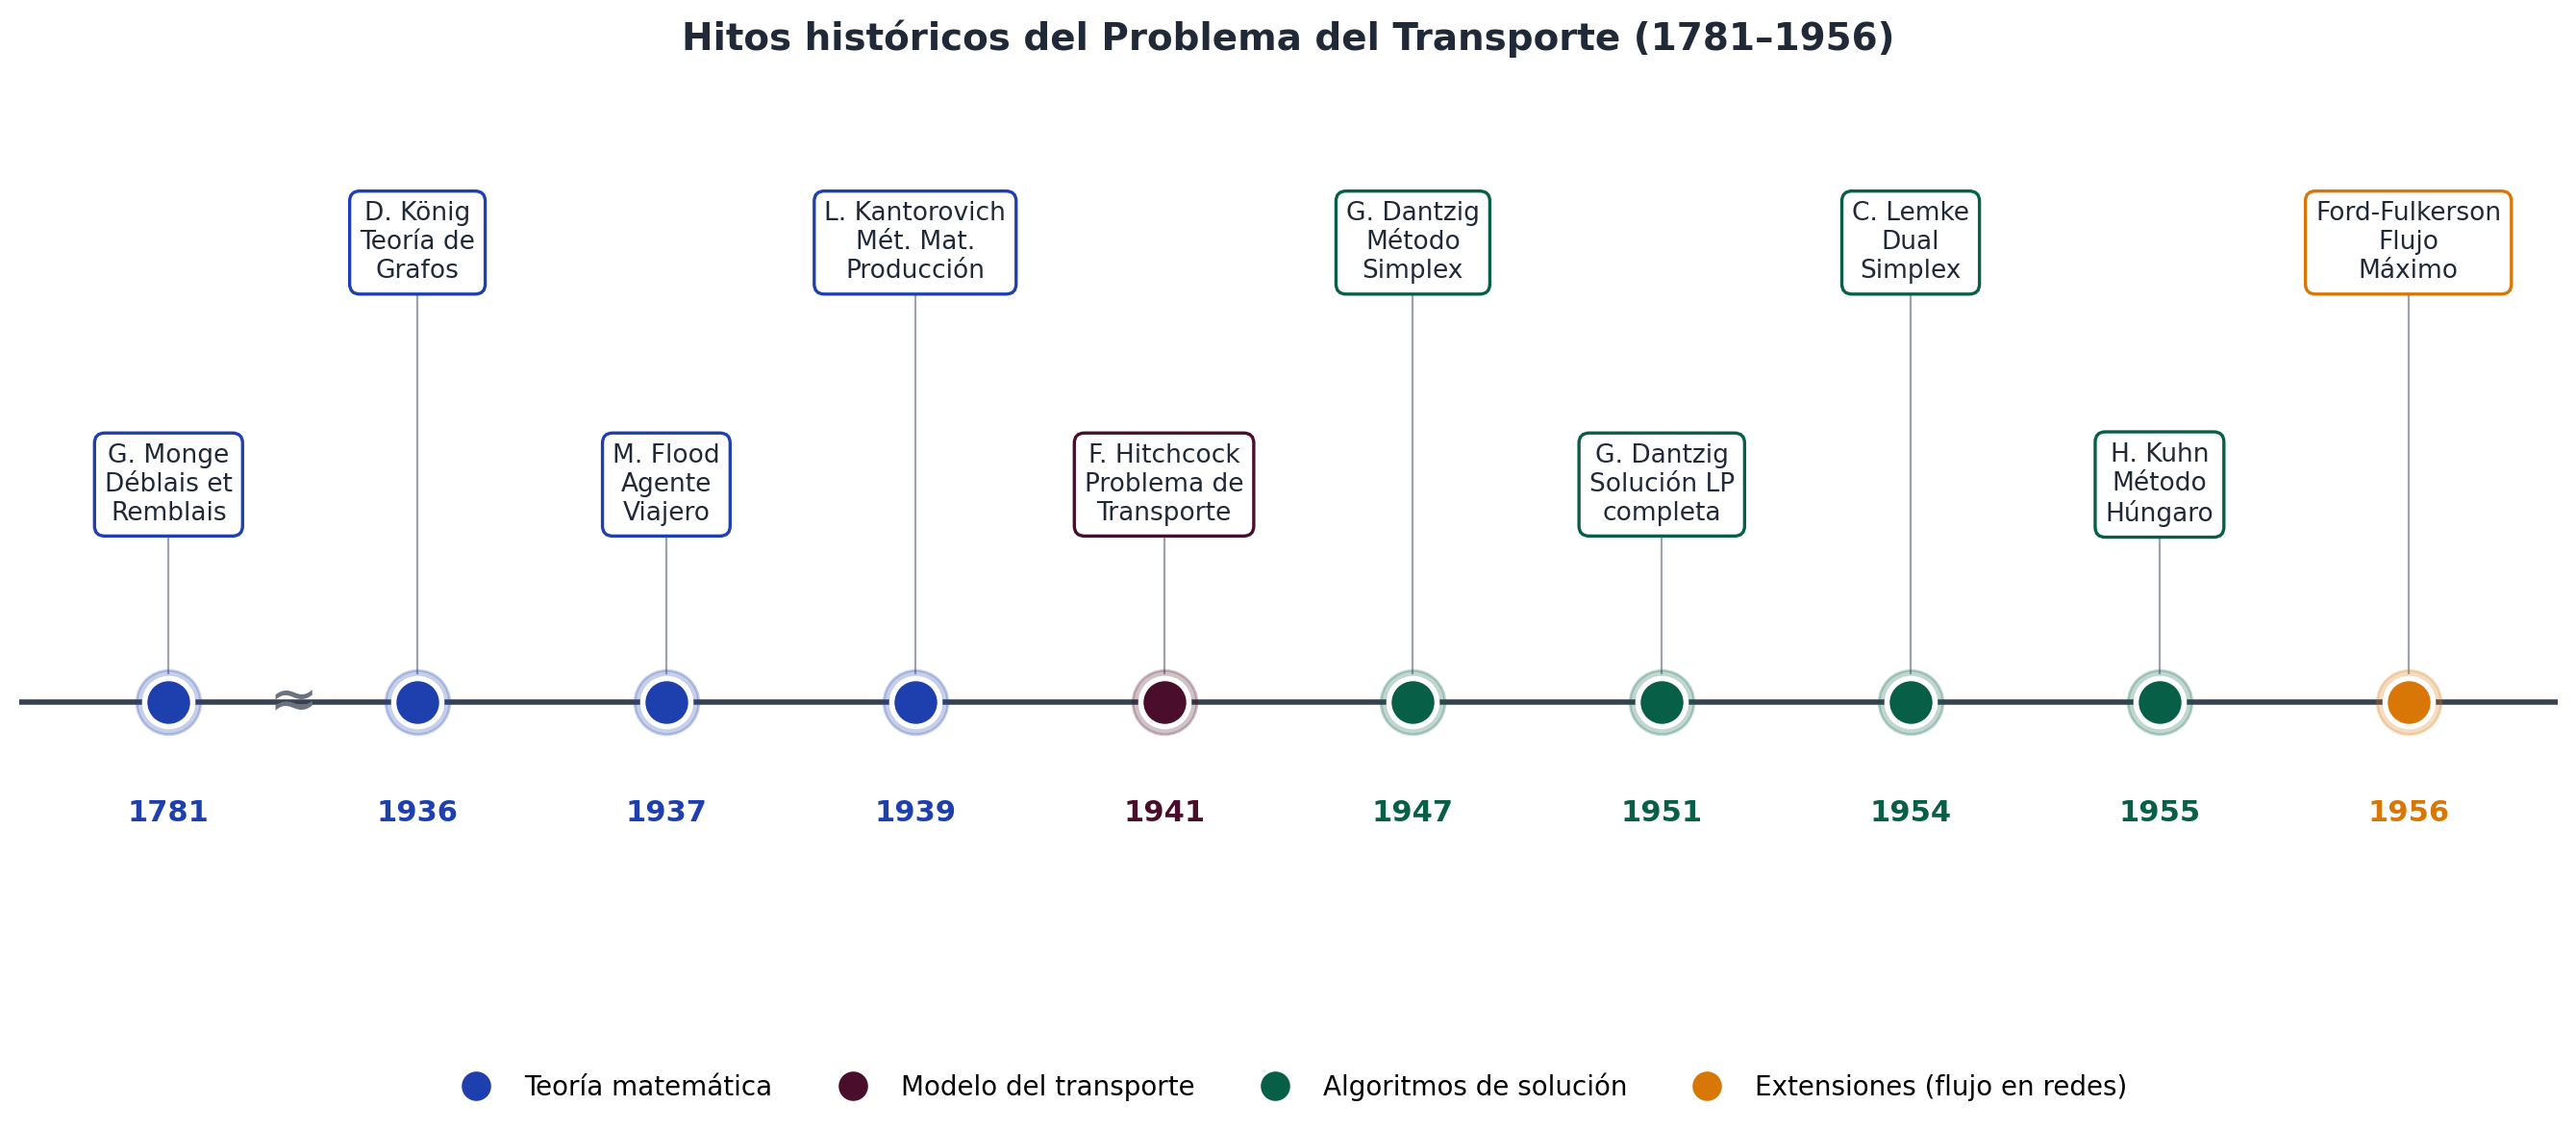
\includegraphics[width=0.95\textwidth]{img/fig1_linea_tiempo.png}
\caption{Hitos históricos del Problema del Transporte. La cronología se divide en tres eras: \emph{Pre-IO} (siglo XVIII, fundamentos geométricos de Monge), \emph{Fundamentos teóricos} (1936--1941, formalización del problema por König, Flood, Kantorovich y Hitchcock) y \emph{Algoritmos y computación} (1947--1956, era del simplex y los flujos en redes). Elaboración propia con base en~[1] y~[2].}
\label{fig:linea_tiempo}
\end{figure*}

\subsection{Modelo geométrico de Monge (1781)}
El trabajo más antiguo conocido sobre el problema se debe a Gaspard Monge, matemático francés del siglo XVIII. En su \emph{Mémoire sur la théorie des déblais et des remblais} (1781), publicado en las memorias de la Academia Francesa de Ciencias, Monge planteó el problema de mover un volumen de tierra desde varios puntos hacia varios destinos minimizando el trabajo total. Su interés provenía de problemas de ingeniería militar relacionados con la construcción de fortificaciones~[1]. Aunque su lenguaje era geométrico ---hablaba de partículas infinitamente pequeñas que se corresponden uno a uno---, su intuición de costos era ya muy similar al actual costeo por tonelada-kilómetro: el precio de mover una partícula es proporcional a su peso y a la distancia recorrida.

\subsection{Teoría de grafos de König (1936)}
Dénes König publicó en 1936 \emph{Theorie der endlichen und unendlichen Graphen}, considerada la primera obra de texto formal dedicada a la teoría de grafos. Su trabajo proporcionó el primer tratamiento sistemático de la teoría de grafos, formalizando conceptos como conectividad, ciclos y caminos que más tarde resultarían esenciales para representar problemas de flujo en redes. En particular, el llamado \textbf{lema de König} —que garantiza la existencia de un camino infinito en cualquier árbol infinito con un número finito de aristas por nodo— es un resultado seminal en la teoría de grafos infinita.

\subsection{Problema del agente viajero de Flood (1937)}
El matemático estadounidense Merrill M. Flood fue uno de los principales impulsores del \textbf{Problema del Agente Viajero} (TSP) en la década de 1930, contribuyendo a su popularización en la comunidad de investigación de operaciones. El TSP consiste en encontrar la ruta más corta para visitar un conjunto de ciudades una sola vez y regresar al origen. Aunque el TSP es un problema de optimización combinatoria fundamentalmente distinto al problema de transporte —este último tiene una estructura de restricciones totalmente unimodular que lo hace ``fácil'' (resoluble en tiempo polinomial), mientras que el TSP es \emph{NP-hard}—, ambos comparten el concepto de minimizar un costo asociado a una red y el trabajo de Flood motivó el desarrollo de métodos de solución para problemas de asignación. Flood llegó al problema desde una aplicación concreta —el enrutamiento de autobuses escolares en Nueva Jersey— y junto con Dresher y Robinson en RAND Corporation impulsó su estudio formal en los años cincuenta.

\subsection{Métodos matemáticos de Kantorovich (1939)}
El matemático ruso Leonid V. Kantorovich propuso en su obra \emph{Métodos matemáticos para la organización y la producción} (1939) la primera formulación de un problema de asignación productiva como un programa lineal. Su enfoque buscaba el uso más eficiente de materiales y mano de obra mediante «valoraciones determinadas objetivamente», antecedentes directos de los precios sombra. Por este aporte recibió el Premio Nobel de Economía en 1975, compartido con T.~C. Koopmans.

\subsection{Modelo de Hitchcock (1941)}
Frank L. Hitchcock publicó en 1941 el artículo «The distribution of a product from several sources to numerous localities», donde formuló de manera explícita el problema de minimizar el costo de distribuir un producto desde varias fábricas hacia un número dado de ciudades. Por su claridad y generalidad, el modelo se conoce desde entonces como el \textbf{Problema de Transporte de Hitchcock}. Trabajos posteriores y de manera independiente fueron desarrollados por Kantorovich (1942) y Koopmans (1947)~[1].

\subsection{Programación lineal y el método simplex (1947)}
George B. Dantzig formalizó en 1947 la programación lineal como disciplina autónoma y desarrolló el \textbf{método simplex}, un algoritmo iterativo que permite resolver problemas con cualquier número de variables. El simplex fue elegido como uno de los diez algoritmos más importantes del siglo XX y sigue siendo, junto con sus variantes, el caballo de batalla de la programación lineal. En 1951 Dantzig adaptó el método para resolver específicamente el problema del transporte~[1].

\subsection{Resolución computacional (década de 1950)}
La primera implementación significativa del problema en una computadora se gestó a inicios de los años cincuenta. En 1951, A.~Orden dirigió un esfuerzo en la computadora SEAC para resolver un modelo de despliegue de la Fuerza Aérea estadounidense, uno de los primeros casos documentados de aplicación de la investigación de operaciones en hardware real. Poco después, en RAND Corporation, Dantzig y Orchard-Hays desarrollaron los primeros códigos especializados, y más tarde aparecieron el método de la esquina noroeste, el método del costo mínimo y el método de aproximación de Vogel.

\subsection{Método dual simplex (1954) y método húngaro (1955)}
Carlton E. Lemke desarrolló en 1954 el \textbf{método dual simplex}, particularmente útil cuando se añaden nuevas restricciones a un problema ya resuelto, pues parte de una solución básica óptima pero infactible y avanza hacia la factibilidad. Un año después, Harold W. Kuhn formalizó el \textbf{método húngaro}, un algoritmo polinomial específico para el problema de asignación ---caso particular del transporte--- basado en la reducción sistemática de la matriz de costos.

\subsection{Algoritmos de flujo en redes (Ford--Fulkerson, 1956)}
L.~R.~Ford y D.~R.~Fulkerson popularizaron en 1956 su algoritmo de flujo máximo, que generalizó el problema del transporte al caso de redes con capacidades en los arcos. Su trabajo abrió la puerta a una familia entera de problemas de optimización combinatoria sobre redes (transbordo, asignación, flujo de costo mínimo) que extienden el modelo clásico.

\subsection{Desarrollos contemporáneos}
En las últimas décadas, la investigación se ha movido hacia variantes que incorporan incertidumbre (programación estocástica), múltiples objetivos (programación multicriterio), múltiples actores con intereses contrapuestos (programación bi-nivel y teoría de juegos) y restricciones combinatorias (programación entera mixta). El modelo gravitacional de distribución de viajes~[4] y los modelos de equilibrio espacial de precios~[5] son ejemplos relevantes de extensiones que conservan la estructura matemática esencial del transporte pero añaden realismo.

% ============================================================
%  3. DESARROLLO Y METODOLOGÍA
% ============================================================
\section{Desarrollo y Metodología}

Esta sección desarrolla el modelo en tres capas: la formulación primal del transportista (3.1), el problema dual del embarcador con los precios sombra (3.2), y la representación topológica como grafo bipartito (3.3).

\subsection{Formulación primal: el enfoque del transportista}

Considérese una red con $m$ orígenes y $n$ destinos. Cada origen $i$ dispone de una oferta $a_i$ y cada destino $j$ requiere una demanda $b_j$. El costo unitario de enviar producto desde el origen $i$ al destino $j$ se denota $c_{ij}$, y la variable de decisión $x_{ij}$ representa la cantidad efectivamente enviada por esa ruta. Se asume el caso balanceado, $\sum a_i = \sum b_j$, en cuyo caso las restricciones se escriben como igualdades~[2]. Nótese que en el caso balanceado, las restricciones de desigualdad $\sum_{j} x_{ij} \leq a_i$ y $\sum_{i} x_{ij} \geq b_j$ son equivalentes a las igualdades (2) y (3), ya que la suma de todas las ofertas es igual a la suma de todas las demandas. Cualquier solución factible que no cumpla una igualdad implicaría un desbalance imposible en el sistema cerrado. El programa lineal asociado es:

\begin{align}
\text{Min}\quad & Z = \sum_{i=1}^{m}\sum_{j=1}^{n} c_{ij}\,x_{ij} \label{eq:primal_obj} \\
\text{s.\,a.}\quad & \sum_{j=1}^{n} x_{ij} = a_i, \quad i = 1,\ldots,m \label{eq:primal_oferta}\\
                   & \sum_{i=1}^{m} x_{ij} = b_j, \quad j = 1,\ldots,n \label{eq:primal_demanda}\\
                   & x_{ij} \geq 0, \quad \forall\, i, j \label{eq:primal_no_neg}
\end{align}

La función objetivo~\eqref{eq:primal_obj} refleja el interés del transportista: minimizar el costo total del plan de distribución. Las restricciones~\eqref{eq:primal_oferta} y~\eqref{eq:primal_demanda} garantizan, respectivamente, que cada origen agote exactamente su oferta y que cada destino reciba exactamente su demanda. La restricción~\eqref{eq:primal_no_neg} impide envíos negativos. En forma matricial compacta, el problema se escribe como
\begin{equation*}
\min \, \mathbf{c}^{\top}\mathbf{x} \quad \text{s.\,a.} \quad A\mathbf{x} = \mathbf{b}, \quad \mathbf{x} \geq \mathbf{0}
\end{equation*}
donde $\mathbf{x}$ es el vector que reúne las $m\cdot n$ variables $x_{ij}$, $\mathbf{c}$ el vector de costos unitarios, $\mathbf{b}$ el vector que concatena ofertas y demandas, y $A$ la matriz de incidencia de tamaño $(m+n) \times (m \cdot n)$, en la cual cada columna —correspondiente a la variable $x_{ij}$— contiene exactamente dos entradas iguales a 1: una en la fila de la restricción de oferta del origen $i$ y otra en la fila de la restricción de demanda del destino $j$. Esta estructura de red le confiere la propiedad de ser \textbf{totalmente unimodular}, lo que garantiza que, si los datos son enteros, la solución básica óptima también será entera.

El modelo es \textbf{balanceado} cuando la oferta total iguala a la demanda total. Cuando no lo es ---cosa que ocurre con frecuencia en la práctica---, se recurre a dos ajustes estándar:

\begin{itemize}
\item Si la oferta excede la demanda, se introduce un \textbf{destino ficticio} con costos unitarios cero que absorbe el excedente sin penalizar la función objetivo.
\item Si la demanda excede la oferta, se introduce un \textbf{origen ficticio} cuya cantidad enviada representa la demanda no satisfecha, a la que normalmente se le asigna un costo de penalización elevado.
\end{itemize}

\subsubsection{Componentes esenciales del modelo}
Los elementos que conviene tener presentes para reproducir cualquier instancia son: las \emph{fuentes} y \emph{destinos} (el grafo bipartito subyacente), los \emph{parámetros} (oferta $a_i$, demanda $b_j$ y costos $c_{ij}$), las \emph{variables de decisión} $x_{ij}$ y, eventualmente, los nodos ficticios para balancear el modelo. El número total de variables del problema crece como $m\cdot n$, mientras que el número de restricciones es $m+n$ (más la no negatividad).

\subsubsection{Procedimiento general de solución}
Cuando se resuelve a mano, el procedimiento clásico consta de tres pasos: (i)~obtener una solución básica factible inicial mediante la esquina noroeste, el costo mínimo o Vogel; (ii)~probar optimalidad mediante el método de los multiplicadores ($u$-$v$), que asocia variables a las restricciones de fila y columna y exige $u_i + v_j = c_{ij}$ para las celdas con flujo; (iii)~si la solución no es óptima, mejorarla construyendo un lazo cerrado para reasignar unidades hacia rutas más baratas. En la práctica moderna, sin embargo, estos pasos los realiza un solver de programación lineal en milisegundos, como se muestra en los ejemplos de la Sección~4.

\subsection{Teoría de dualidad y precios sombra}

A cada restricción del primal le corresponde una variable del dual. Asociando a las restricciones de oferta~\eqref{eq:primal_oferta} las variables $u_i$ y a las de demanda~\eqref{eq:primal_demanda} las variables $v_j$, el dual del problema (1)--(4) resulta~[3]:

\begin{align}
\text{Max}\quad & W = \sum_{i} a_i u_i + \sum_{j} b_j v_j \label{eq:dual_obj}\\
\text{s.\,a.}\quad & u_i + v_j \leq c_{ij}, \quad \forall\, i, j \label{eq:dual_rest}\\
                   & u_i,\, v_j \text{ irrestrictas en signo} \label{eq:dual_no_sign}
\end{align}

En forma matricial compacta, el dual se escribe como
$\max\, \mathbf{b}^{\top}\mathbf{y}$ sujeto a $A^{\top}\mathbf{y} \leq \mathbf{c}$, donde $\mathbf{y} = (u_1,\ldots,u_m, v_1,\ldots,v_n)$ y $A$ es la misma matriz de incidencia del primal.

\subsubsection{Interpretación económica}
Mientras el primal representa al \emph{transportista} que minimiza costos, el dual representa al \emph{embarcador} que compra el producto en los orígenes y lo vende en los destinos buscando maximizar la utilidad de la operación~[3]. Las variables duales adquieren entonces un significado económico muy concreto:

\begin{itemize}
\item $u_i$ \textbf{--- precio sombra en el origen:} valor marginal de contar con una unidad adicional de oferta en el origen $i$. Mide el impacto en el costo óptimo total: $\partial Z^*/\partial a_i = u_i^*$.
\item $v_j$ \textbf{--- precio sombra en el destino:} costo marginal de satisfacer una unidad adicional de demanda en el destino $j$. Se cumple $\partial Z^*/\partial b_j = v_j^*$.
\end{itemize}

La restricción~\eqref{eq:dual_rest}, $u_i + v_j \leq c_{ij}$, expresa una condición de equilibrio espacial de precios: el valor marginal de enviar una unidad del origen $i$ al destino $j$ no puede exceder el costo de hacerlo. Si $u_i + v_j < c_{ij}$, resulta más costoso mover el producto que el valor que genera, por lo que la ruta permanece inactiva. Cournot ya había formalizado este principio de equilibrio espacial en 1838: «un artículo capaz de ser transportado debe fluir del mercado donde su valor es menor al mercado donde su valor es más grande, hasta que la diferencia en valor, de un mercado al otro, no represente más que el costo del transporte»~[5].

\subsubsection{Holgura complementaria}
La teoría de dualidad establece que en la solución óptima se cumple para cada par $(i, j)$:
\begin{equation}
x_{ij}^* \cdot (c_{ij} - u_i^* - v_j^*) = 0 \label{eq:holgura}
\end{equation}

De esta ecuación se desprenden dos casos lógicos. Primero, si la ruta es \textbf{activa} ($x_{ij}^* > 0$), entonces $u_i^* + v_j^* = c_{ij}$: el precio sombra en el destino es exactamente el precio sombra en el origen más el costo de transporte. Esto constituye un equilibrio de mercado perfecto. Segundo, si la ruta es \textbf{deficitaria} ($u_i^* + v_j^* < c_{ij}$), entonces necesariamente $x_{ij}^* = 0$: trasladar producto por esa ruta destruiría valor, así que el flujo se anula. La \textbf{Figura~\ref{fig:primal_dual}} resume gráficamente la dualidad primal-dual.

\begin{figure*}[!t]
\centering
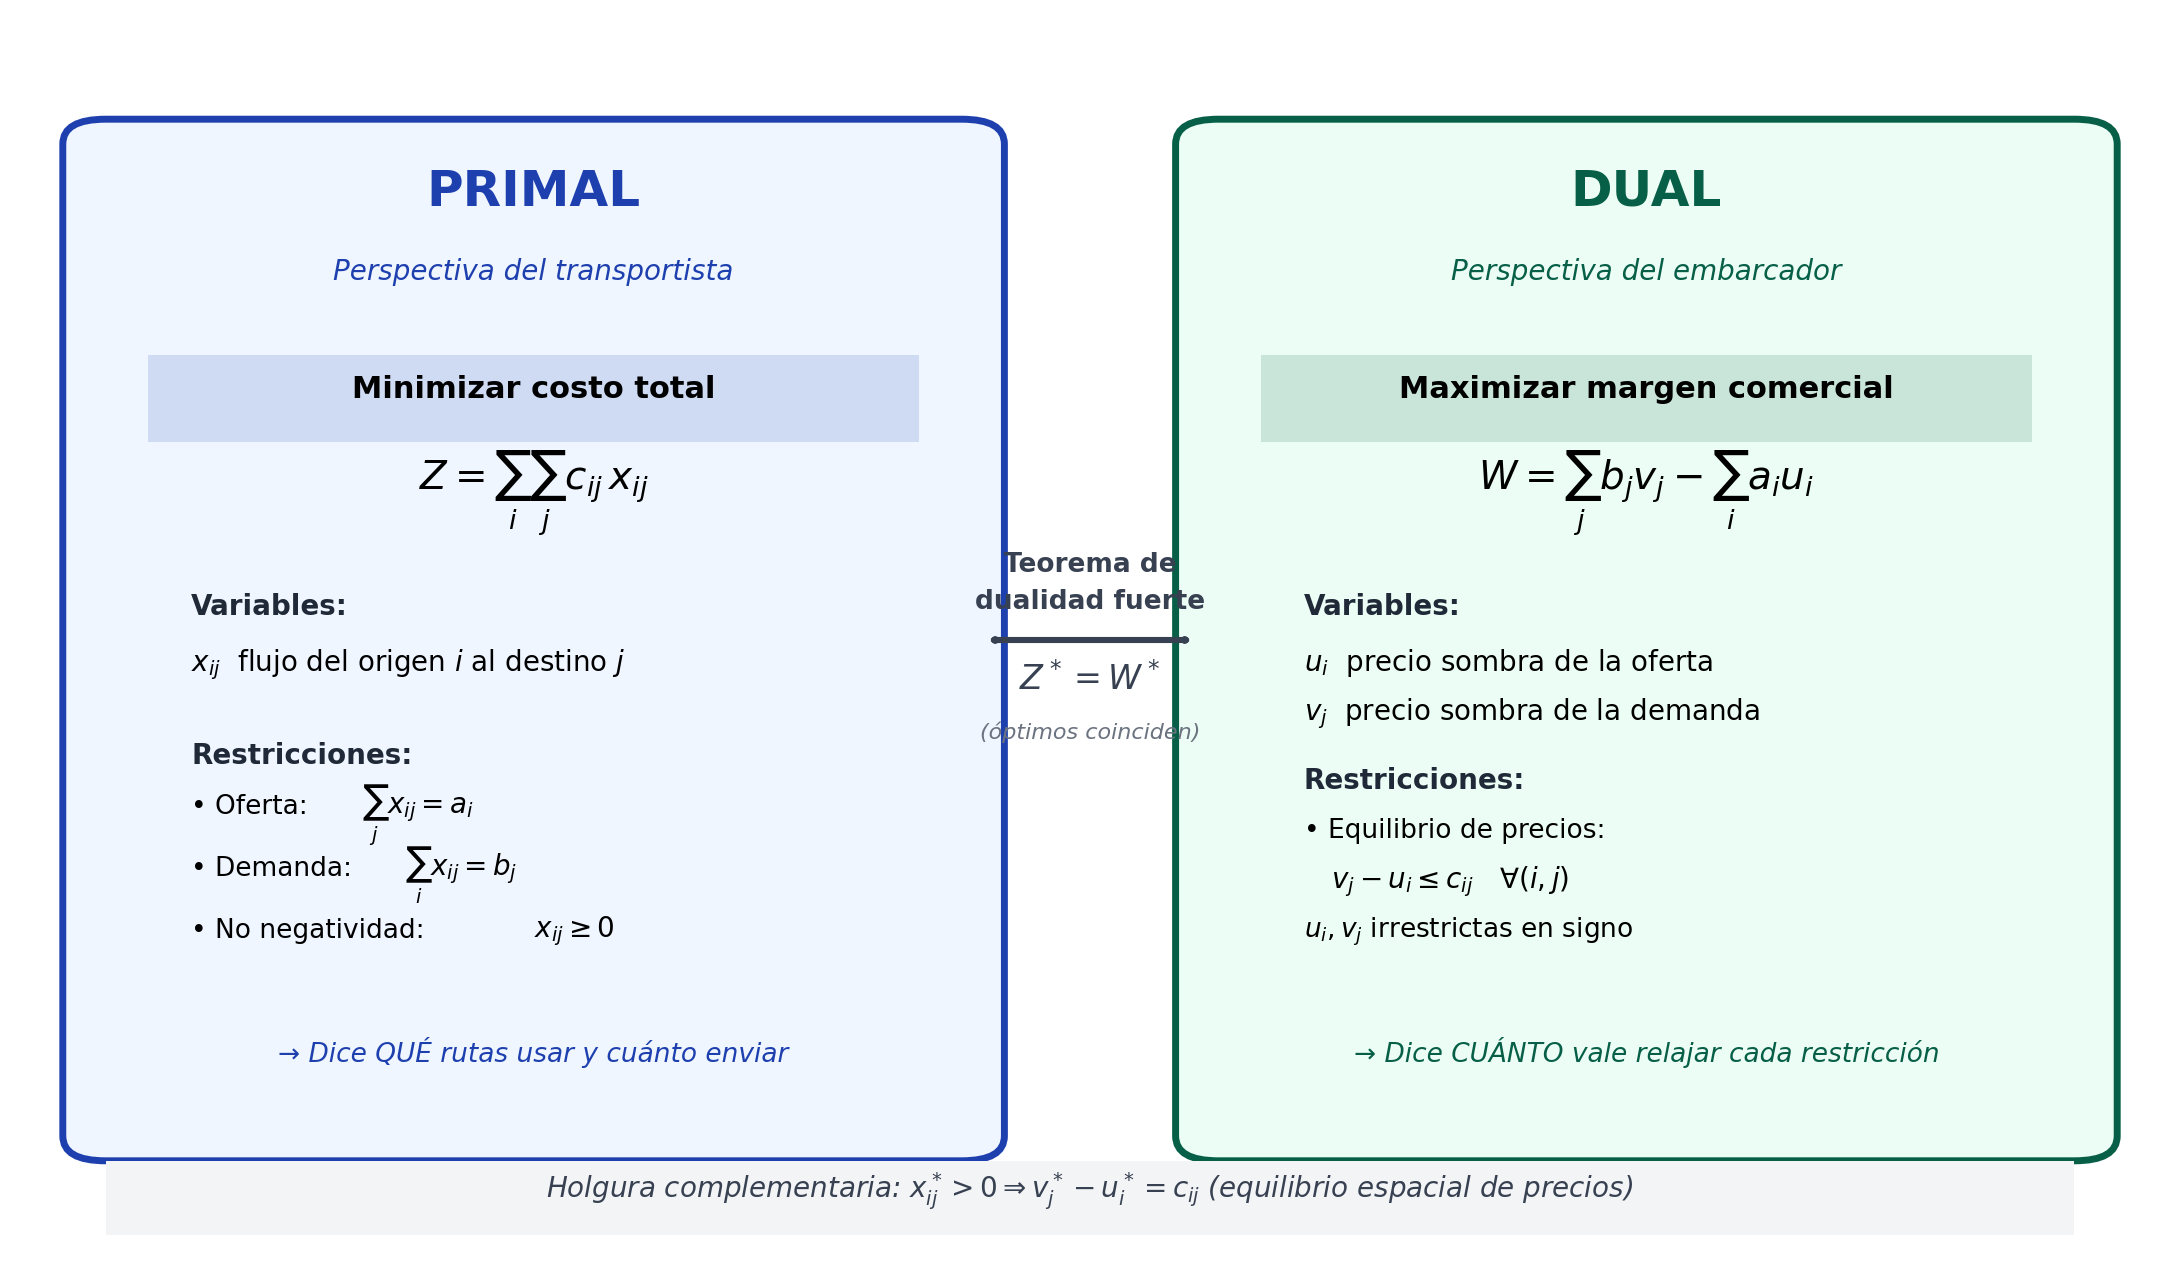
\includegraphics[width=0.92\textwidth]{img/fig2_primal_dual.png}
\caption{Esquema integral de la relación primal--dual. El problema primal busca minimizar el costo total desde la perspectiva del transportista, mientras que su dual busca maximizar la suma de los precios sombra ponderados por oferta y demanda. La teoría de dualidad fuerte garantiza que ambos programas alcanzan el mismo valor en el óptimo ($Z^* = W^*$). La condición de holgura complementaria, mostrada en la banda inferior, conecta las soluciones primal y dual: cuando una ruta tiene flujo positivo, el precio sombra en el destino iguala al del origen más el costo de transporte, reproduciendo el principio de equilibrio espacial.}
\label{fig:primal_dual}
\end{figure*}

\subsection{Representación mediante grafos bipartitos}

El problema admite una representación natural como un \textbf{grafo bipartito dirigido} $G = (V, E)$ donde el conjunto de vértices se parte en dos subconjuntos disjuntos: orígenes $S$ y destinos $D$. Cada origen $i$ se asocia a una divergencia de flujo positiva ($+a_i$), y cada destino $j$ a una divergencia negativa ($-b_j$). Las aristas conectan únicamente nodos de $S$ con nodos de $D$; no existen aristas entre dos orígenes ni entre dos destinos. La \textbf{Figura~\ref{fig:grafo_generico}} ilustra esta estructura para un caso pequeño con dos orígenes y tres destinos.

\begin{figure}[!t]
\centering
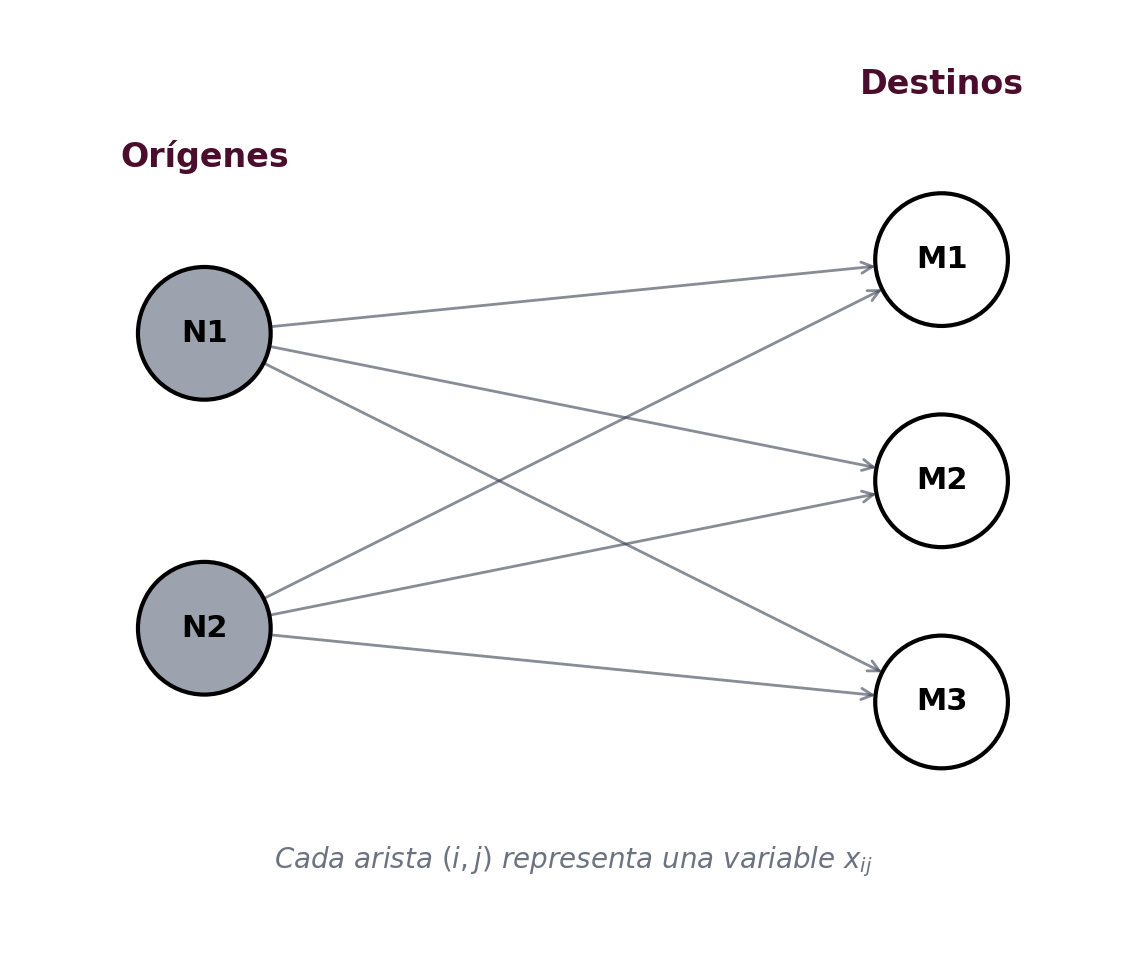
\includegraphics[width=\columnwidth]{img/fig3_grafo_generico.png}
\caption{Grafo bipartito genérico de un problema de transporte con dos orígenes ($N_1$, $N_2$) y tres destinos ($M_1$, $M_2$, $M_3$). Las aristas dirigidas $(i,j) \in E$ con costo $c_{ij}$ conectan exclusivamente nodos de $S$ con nodos de $D$; el número total de aristas $|S|\times|D|$ coincide con el número de variables de decisión $x_{ij}$ del programa lineal. Adaptado de~[3].}
\label{fig:grafo_generico}
\end{figure}

Existe una correspondencia exacta entre la estructura del grafo y la estructura algebraica del problema: \textbf{el número de aristas del grafo bipartito completo es igual al número de variables de decisión} del programa lineal, es decir, $m\cdot n$. Cada variable $x_{ij}$ representa el flujo que circula por la arista $(i, j)$.

Una propiedad fundamental es que las restricciones de oferta y demanda en el caso balanceado contienen una ecuación redundante (la suma de las ofertas iguala a la suma de las demandas), por lo que el rango efectivo del sistema es $m+n-1$. Esto implica que la solución óptima activará a lo sumo $m+n-1$ aristas, las cuales formarán topológicamente un \textbf{árbol de expansión}: una estructura sin ciclos que conecta todos los nodos relevantes. Esta característica garantiza que no haya rutas redundantes en el plan óptimo. Adicionalmente, la matriz de coeficientes asociada a este tipo de redes es \emph{totalmente unimodular}, lo que asegura que la solución óptima de la relajación lineal sea entera siempre que la oferta y la demanda lo sean.

\subsubsection{Implementación computacional de referencia}
A continuación se presenta una implementación genérica que materializa los tres elementos teóricos discutidos hasta aquí: la formulación primal (1)--(4), la extracción de los precios sombra del dual (Sección~3.2) y la visualización topológica como grafo bipartito. El código emplea \texttt{PuLP} para la optimización y \texttt{NetworkX} para el dibujo del árbol de expansión óptimo. Sirve como plantilla que los ejemplos de la Sección~4 particularizan con datos reales:

\begin{lstlisting}
"""
Analisis Computacional del Problema de
Transporte Bipartito.
Optimizacion Primal-Dual (PuLP), Extraccion
de Precios Sombra y Topologia (NetworkX).
"""
import pulp
import networkx as nx
import matplotlib.pyplot as plt

def instanciar_y_resolver_transporte():
    # 1. Definicion de Parametros
    origenes = ["Planta_A", "Planta_B", "Planta_C"]
    oferta = {"Planta_A": 2000, "Planta_B": 1500,
              "Planta_C": 1000}

    destinos = ["Mercado_1", "Mercado_2",
                "Mercado_3", "Mercado_4"]
    demanda = {"Mercado_1": 1300, "Mercado_2": 1800,
               "Mercado_3": 900,  "Mercado_4": 500}

    costos = {
      "Planta_A": {"Mercado_1":10, "Mercado_2":15,
                   "Mercado_3":20, "Mercado_4":12},
      "Planta_B": {"Mercado_1":12, "Mercado_2":10,
                   "Mercado_3":15, "Mercado_4":18},
      "Planta_C": {"Mercado_1":15, "Mercado_2":25,
                   "Mercado_3":10, "Mercado_4":14},
    }

    # 2. Inicializacion del Modelo Primal
    modelo = pulp.LpProblem("Modelo_Transporte",
                            pulp.LpMinimize)

    # 3. Aristas equivalentes (variables x_ij)
    rutas = [(i, j) for i in origenes
                    for j in destinos]
    flujos = pulp.LpVariable.dicts(
        "Carga", rutas, lowBound=0,
        cat=pulp.LpContinuous)

    # 4. Funcion objetivo Z
    modelo += pulp.lpSum(flujos[(i, j)]*costos[i][j]
                         for (i, j) in rutas)

    # 5. Balance de masa (oferta y demanda)
    for i in origenes:
        modelo += (pulp.lpSum(flujos[(i, j)]
                   for j in destinos) == oferta[i],
                   f"Oferta_{i}")
    for j in destinos:
        modelo += (pulp.lpSum(flujos[(i, j)]
                   for i in origenes) == demanda[j],
                   f"Demanda_{j}")

    # 6. Resolucion
    modelo.solve(pulp.PULP_CBC_CMD(msg=False))
    print(f"Z* = ${pulp.value(modelo.objective):,.2f}")

    # 7. Aristas activas y precios sombra
    activas = []
    for (i, j) in rutas:
        v = flujos[(i, j)].varValue
        if v and v > 0:
            print(f"{i} -> {j}: {v} unidades")
            activas.append((i, j, v))

    print("--- Precios sombra ---")
    for i in origenes:
        u_i = modelo.constraints[f"Oferta_{i}"].pi
        print(f"u_{i} = {u_i}")
    for j in destinos:
        v_j = modelo.constraints[f"Demanda_{j}"].pi
        print(f"v_{j} = {v_j}")

    # 8. Grafo bipartito del arbol optimo
    generar_grafo_bipartito(origenes, destinos,
                            activas)

def generar_grafo_bipartito(origenes, destinos,
                             aristas):
    """Visualiza el arbol de expansion optimo."""
    G = nx.DiGraph()
    G.add_nodes_from(origenes, bipartite=0)
    G.add_nodes_from(destinos, bipartite=1)
    for (u, v, flujo) in aristas:
        G.add_edge(u, v, weight=flujo)

    plt.figure(figsize=(10, 6))
    pos = nx.bipartite_layout(G, origenes)
    nx.draw_networkx_nodes(G, pos, nodelist=origenes,
        node_color='skyblue', node_size=2000)
    nx.draw_networkx_nodes(G, pos, nodelist=destinos,
        node_color='lightgreen', node_size=2000)
    nx.draw_networkx_edges(G, pos, arrowstyle='-|>',
        edge_color='gray', width=2)
    nx.draw_networkx_labels(G, pos, font_size=10,
        font_weight='bold')

    etiquetas = {(u, v): f"{flujo}"
                 for u, v, flujo in aristas}
    nx.draw_networkx_edge_labels(G, pos,
        edge_labels=etiquetas, font_size=9)

    plt.title("Grafo Bipartito: Arbol de "
              "Expansion Optimo", fontsize=14)
    plt.axis('off')
    plt.show()

if __name__ == "__main__":
    instanciar_y_resolver_transporte()
\end{lstlisting}

\noindent Esta implementación de referencia es deliberadamente genérica: cualquier instancia concreta del problema se obtiene reemplazando los diccionarios de \texttt{oferta}, \texttt{demanda} y \texttt{costos}. Los dos ejemplos de la Sección~4 siguen exactamente este patrón, agregando en el segundo caso restricciones de capacidad, bloqueos y prioridades sobre las variables.

% ============================================================
%  4. EJEMPLOS PRÁCTICOS RESUELTOS
% ============================================================
\section{Ejemplos Prácticos Resueltos}

Esta sección presenta dos ejemplos numéricos del Problema del Transporte resueltos íntegramente con la biblioteca \textbf{PuLP} de Python. El Ejemplo~1 (Sección~4.1) modela una red de logística de última milla en un escenario de e-commerce balanceado. El Ejemplo~2 (Sección~4.2) extiende el modelo anterior con restricciones adicionales que reflejan situaciones operativas reales: una ruta físicamente bloqueada, capacidades máximas en ciertas tuberías y una condición de prioridad obligatoria. Ambos ejemplos permiten apreciar la flexibilidad del modelo y la utilidad práctica del análisis de los precios sombra.

\subsection{Ejemplo 1: Logística de última milla en e-commerce}

\subsubsection{Caso de estudio}
Durante la temporada comercial del «Buen Fin 2026», la empresa Mercado Libre (en adelante, «la empresa») proyecta un pico histórico de ventas para el lanzamiento del iPhone~18. Para garantizar el cumplimiento de las entregas bajo la modalidad «Full» (entrega al día siguiente), la compañía requiere preposicionar su inventario de manera estratégica antes de que comience el evento.

La empresa cuenta con tres Mega Centros de Distribución (orígenes) que en conjunto tienen almacenados 120 lotes del producto, donde un lote equivale a 100 unidades. Estos lotes deben distribuirse a cinco Centros de Última Milla (destinos), cuya demanda proyectada suma exactamente 120 lotes. Como la oferta total iguala a la demanda total, el sistema se clasifica como un \textbf{problema de transporte balanceado}~[2]. Las \textbf{Tablas I y II} resumen oferta y demanda; la \textbf{Tabla III} presenta la matriz de costos de transporte terrestre, expresados en pesos mexicanos por lote.

\begin{table}[!h]
\caption{Oferta disponible por Mega Centro (orígenes).}
\centering
\small
\begin{tabular}{c l r}
\arrayrulecolor{infotec}\toprule
\rowcolor{infotec}\textcolor{white}{\textbf{Origen $i$}} & \textcolor{white}{\textbf{Ubicación}} & \textcolor{white}{\textbf{Lotes ($a_i$)}} \\
\midrule
1 & Cuautitlán Izcalli & 40 \\
2 & Monterrey & 35 \\
3 & Guadalajara & 45 \\
\midrule
\multicolumn{2}{l}{\textbf{Total}} & \textbf{120} \\
\bottomrule
\end{tabular}
\arrayrulecolor{black}
\end{table}

\begin{table}[!h]
\caption{Demanda requerida por Centro de Última Milla (destinos).}
\centering
\small
\begin{tabular}{c l r}
\arrayrulecolor{infotec}\toprule
\rowcolor{infotec}\textcolor{white}{\textbf{Destino $j$}} & \textcolor{white}{\textbf{Ubicación}} & \textcolor{white}{\textbf{Lotes ($b_j$)}} \\
\midrule
1 & Tijuana & 20 \\
2 & Puebla & 25 \\
3 & Querétaro & 30 \\
4 & Mérida & 15 \\
5 & Hermosillo & 30 \\
\midrule
\multicolumn{2}{l}{\textbf{Total}} & \textbf{120} \\
\bottomrule
\end{tabular}
\arrayrulecolor{black}
\end{table}

\begin{table}[!h]
\caption{Matriz de costos $c_{ij}$ en MXN por lote.}
\centering
\footnotesize
\begin{tabular}{l r r r r r}
\arrayrulecolor{infotec}\toprule
\rowcolor{infotec}\textcolor{white}{\textbf{Origen}} & \textcolor{white}{\textbf{Tij.}} & \textcolor{white}{\textbf{Pue.}} & \textcolor{white}{\textbf{Qro.}} & \textcolor{white}{\textbf{Mér.}} & \textcolor{white}{\textbf{Hmo.}} \\
\midrule
Cuautitlán  & 2,800 & 500   & 700   & 3,200 & 2,500 \\
Monterrey   & 2,400 & 1,800 & 1,200 & 3,800 & 1,600 \\
Guadalajara & 2,200 & 1,100 & 600   & 3,500 & 1,900 \\
\bottomrule
\end{tabular}
\arrayrulecolor{black}
\end{table}

\subsubsection{Representación en grafo bipartito}
El sistema se modela mediante un grafo bipartito dirigido con tres nodos de origen y cinco de destino, lo que da un total de \textbf{15 aristas} posibles ---es decir, 15 variables de decisión $x_{ij}$. La \textbf{Figura~\ref{fig:grafo_ej1}} muestra todas las rutas potenciales antes de que el modelo decida cuáles activar. Por la regla de redes mencionada en la Sección~3.3, la solución óptima activará a lo sumo $m+n-1 = 3+5-1 = 7$ rutas; en este caso particular, el algoritmo encontrará el óptimo con sólo 6 rutas activas.

\begin{figure}[!h]
\centering
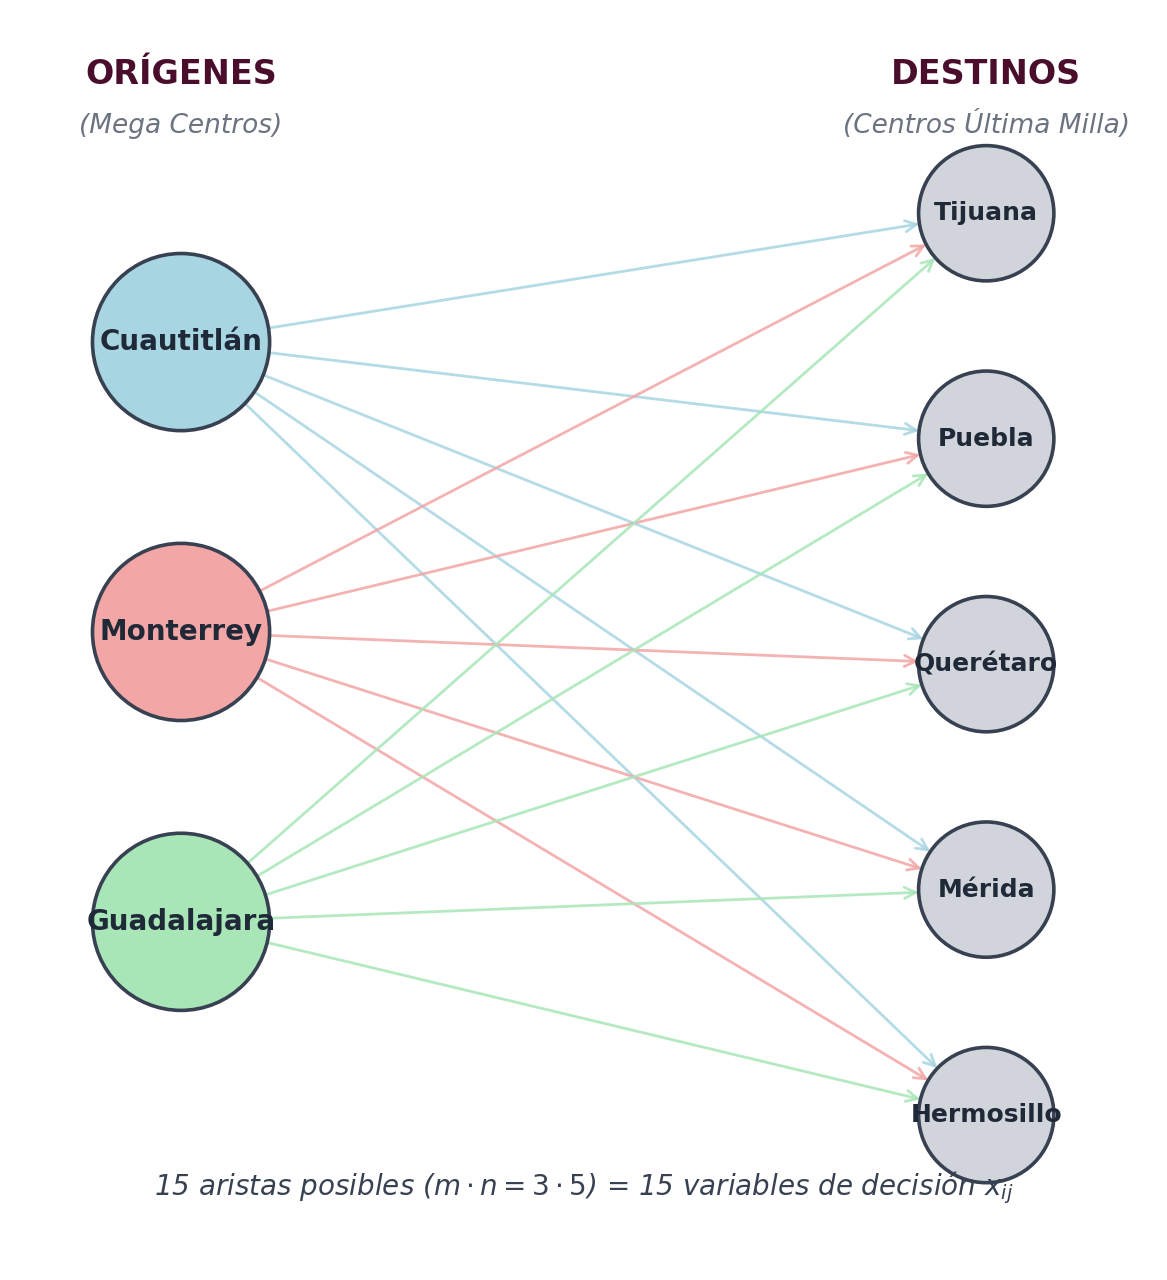
\includegraphics[width=\columnwidth]{img/fig4_grafo_ej1.png}
\caption{Grafo bipartito completo del Ejemplo~1: tres orígenes (Cuautitlán, Monterrey, Guadalajara, identificados por color) conectados con cinco destinos (en gris) mediante 15 aristas posibles. Cada arista representa una variable de decisión $x_{ij}$. La teoría de redes garantiza que la solución óptima activará a lo sumo $m+n-1=7$ aristas, formando un árbol de expansión.}
\label{fig:grafo_ej1}
\end{figure}

\subsubsection{Formulación matemática}
Sea $x_{ij}$ la cantidad de lotes enviados desde el origen $i$ al destino $j$, con $i \in \{1,2,3\}$ y $j \in \{1,\ldots,5\}$. La función objetivo, particularizando la fórmula (1) con los costos de la Tabla~III, queda:

\begin{align*}
\text{Min}\; Z =\;& 2800 x_{11} + 500 x_{12} + 700 x_{13} +\\
                  & 3200 x_{14} + 2500 x_{15} + 2400 x_{21} +\\
                  & 1800 x_{22} + 1200 x_{23} + 3800 x_{24} +\\
                  & 1600 x_{25} + 2200 x_{31} + 1100 x_{32} +\\
                  & 600 x_{33} + 3500 x_{34} + 1900 x_{35}
\end{align*}

Con las cinco restricciones de oferta y demanda balanceadas (omitidas aquí por brevedad), y la condición de no negatividad $x_{ij} \geq 0$ para todo $(i, j)$.

\subsubsection{Resolución computacional}
Por la dimensionalidad del modelo (15 variables, 8 restricciones de igualdad), la resolución manual sería tediosa pero perfectamente factible. En la práctica se utiliza la biblioteca \textbf{PuLP}, un modelador de programación lineal en Python que se conecta automáticamente con solvers como CBC o GLPK. PuLP permite declarar la función objetivo y las restricciones con una sintaxis natural y devuelve, además del plan óptimo, los precios sombra como subproducto del solver. El siguiente fragmento contiene el código completo:

\begin{lstlisting}
import pulp

origenes  = ['Cuautitlan', 'Monterrey',
             'Guadalajara']
destinos  = ['Tijuana', 'Puebla', 'Queretaro',
             'Merida', 'Hermosillo']
oferta    = {'Cuautitlan': 40, 'Monterrey': 35,
             'Guadalajara': 45}
demanda   = {'Tijuana': 20, 'Puebla': 25,
             'Queretaro': 30, 'Merida': 15,
             'Hermosillo': 30}

costos = {
  'Cuautitlan':  {'Tijuana':2800,'Puebla':500,
                  'Queretaro':700,'Merida':3200,
                  'Hermosillo':2500},
  'Monterrey':   {'Tijuana':2400,'Puebla':1800,
                  'Queretaro':1200,'Merida':3800,
                  'Hermosillo':1600},
  'Guadalajara': {'Tijuana':2200,'Puebla':1100,
                  'Queretaro':600,'Merida':3500,
                  'Hermosillo':1900},
}

prob  = pulp.LpProblem("Logistica",
                       pulp.LpMinimize)
rutas = [(o, d) for o in origenes
                for d in destinos]
x = pulp.LpVariable.dicts("Ruta",
                          (origenes, destinos),
                          lowBound=0)

# Funcion objetivo
prob += pulp.lpSum(x[o][d] * costos[o][d]
                   for (o, d) in rutas)

# Restricciones de oferta
for o in origenes:
    prob += pulp.lpSum(x[o][d]
              for d in destinos) == oferta[o]

# Restricciones de demanda
for d in destinos:
    prob += pulp.lpSum(x[o][d]
              for o in origenes) == demanda[d]

prob.solve(pulp.PULP_CBC_CMD(msg=False))
print(f"Z* = ${pulp.value(prob.objective):,.0f}")
\end{lstlisting}

Al ejecutar el script, el solver CBC encuentra la solución óptima global en aproximadamente 0.05~segundos. La salida del programa es:

\begin{lstlisting}[style=terminalStyle]
Z* = $171,500
Ruta_Cuautitlan_Merida:    15 lotes
Ruta_Cuautitlan_Puebla:    25 lotes
Ruta_Guadalajara_Queretaro: 30 lotes
Ruta_Guadalajara_Tijuana:  15 lotes
Ruta_Monterrey_Hermosillo: 30 lotes
Ruta_Monterrey_Tijuana:     5 lotes
\end{lstlisting}

\subsubsection{Resultados e interpretación}
El costo mínimo del plan logístico es $\boldsymbol{Z^* = \$171{,}500\text{~MXN}}$. La \textbf{Figura~\ref{fig:matriz_ej1}} muestra la matriz de asignación óptima: las celdas resaltadas corresponden a las rutas activas, con el flujo asignado, el costo unitario y el subtotal de cada ruta. La \textbf{Figura~\ref{fig:intuicion_vs_optimo}} compara este plan óptimo con un plan ``intuitivo'' que un planeador humano podría haber diseñado siguiendo la lógica geográfica de proximidad, evidenciando un ahorro de \$7{,}000 (3.9\,\%) gracias a la optimización global. De las 15 rutas posibles del planteamiento inicial, el modelo descartó 9 (asignándoles flujo cero), dejando sólo las 6 que minimizan el costo total. La \textbf{Figura~\ref{fig:arbol_expansion}} visualiza estas 6 rutas como un árbol de expansión, materializando la propiedad teórica de que la solución óptima activa a lo sumo $m+n-1 = 7$ aristas.

\begin{figure*}[!t]
\centering
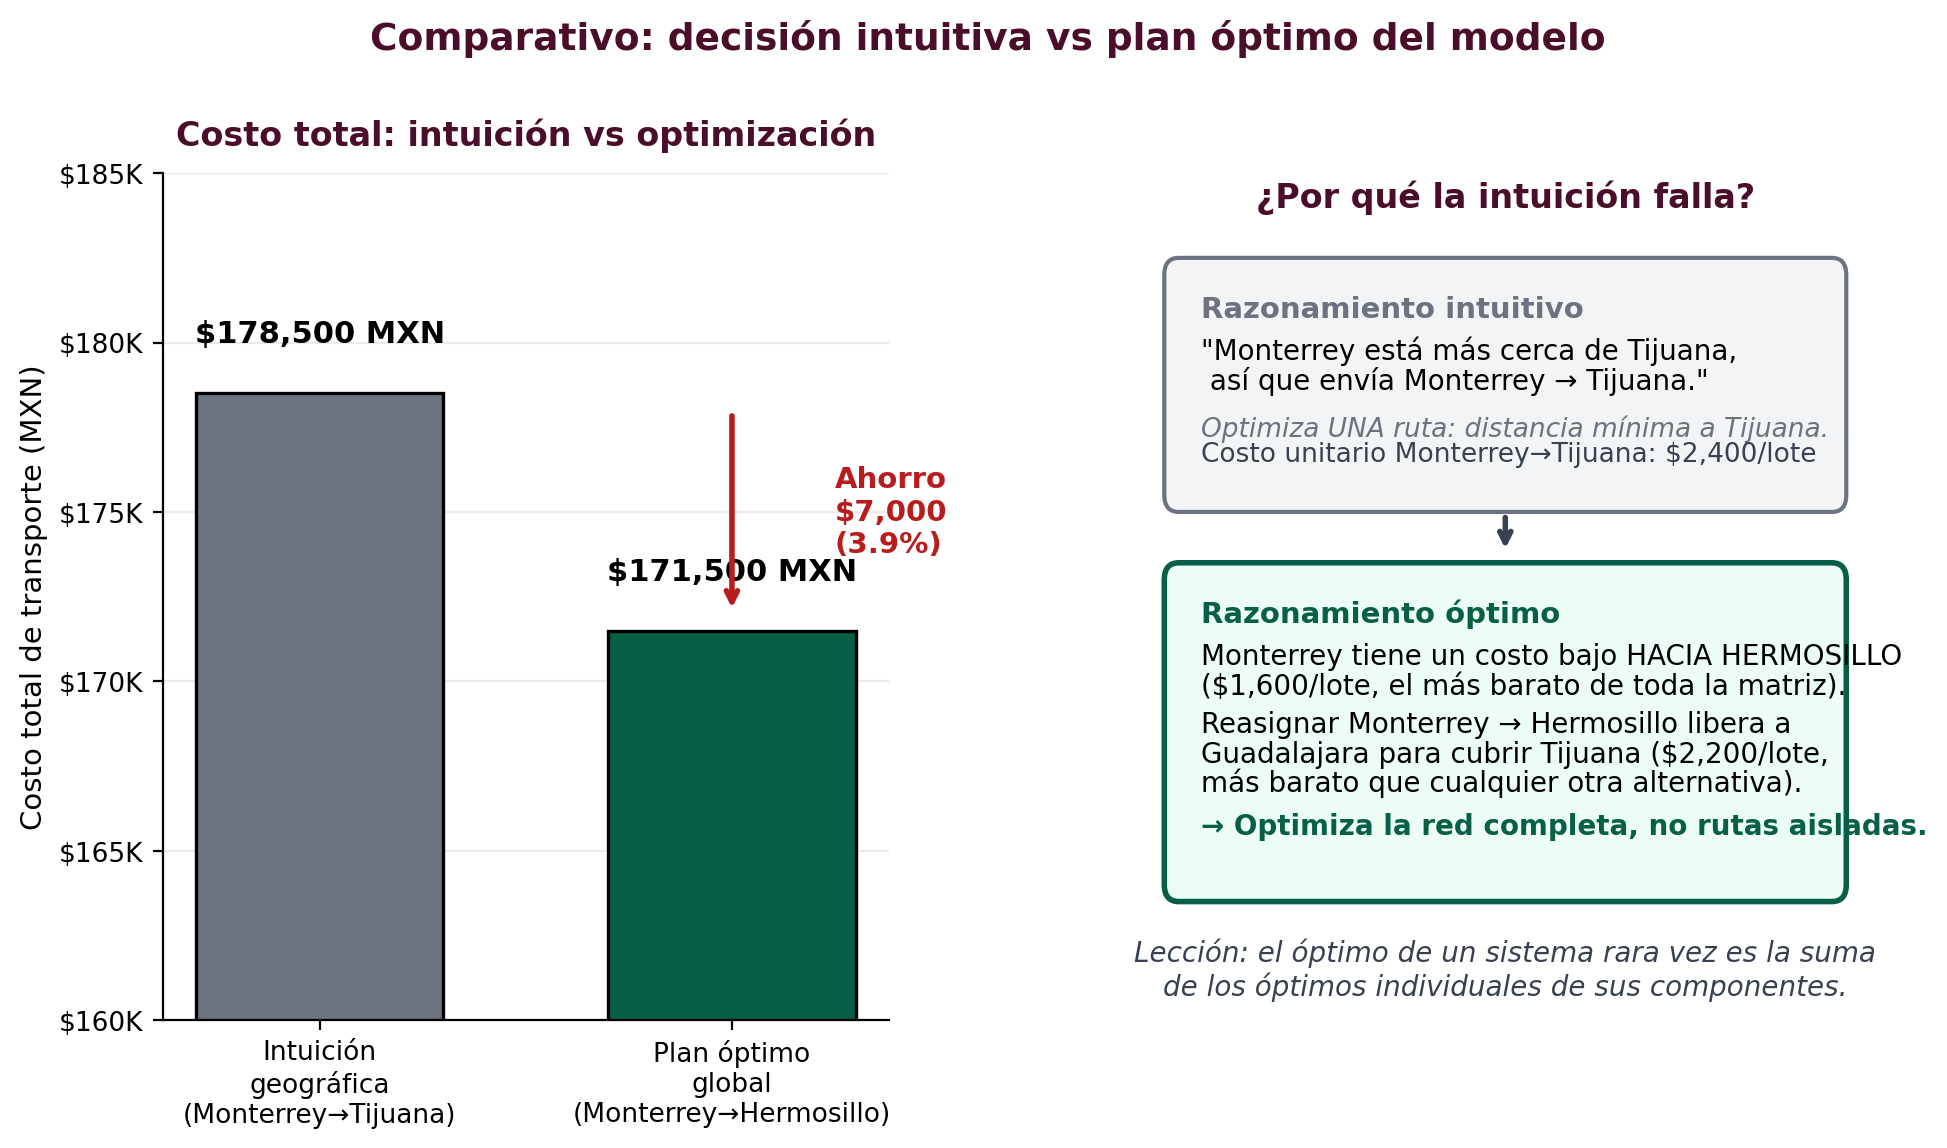
\includegraphics[width=0.85\textwidth]{img/fig5_intuicion_vs_optimo.png}
\caption{Comparativo \emph{intuición vs.\ optimización} para el Ejemplo~1. \textbf{Izquierda:} el plan ``intuitivo'' que asigna todo Tijuana a Monterrey (la ciudad geográficamente más cercana) cuesta \$178{,}500 MXN, mientras que el plan óptimo del modelo cuesta \$171{,}500, un ahorro de \$7{,}000 (3.9\,\%). \textbf{Derecha:} explicación del razonamiento detrás de cada estrategia. El modelo redirige inventario para evitar el costo unitario más alto de Monterrey~$\to$~Tijuana (\$2{,}400/lote) en favor de Guadalajara~$\to$~Tijuana (\$2{,}200/lote), liberando capacidad de Monterrey hacia Hermosillo. La conclusión gerencial es directa: minimizar el costo de una ruta aislada no garantiza minimizar el costo total de la red.}
\label{fig:intuicion_vs_optimo}
\end{figure*}

\begin{figure*}[!t]
\centering
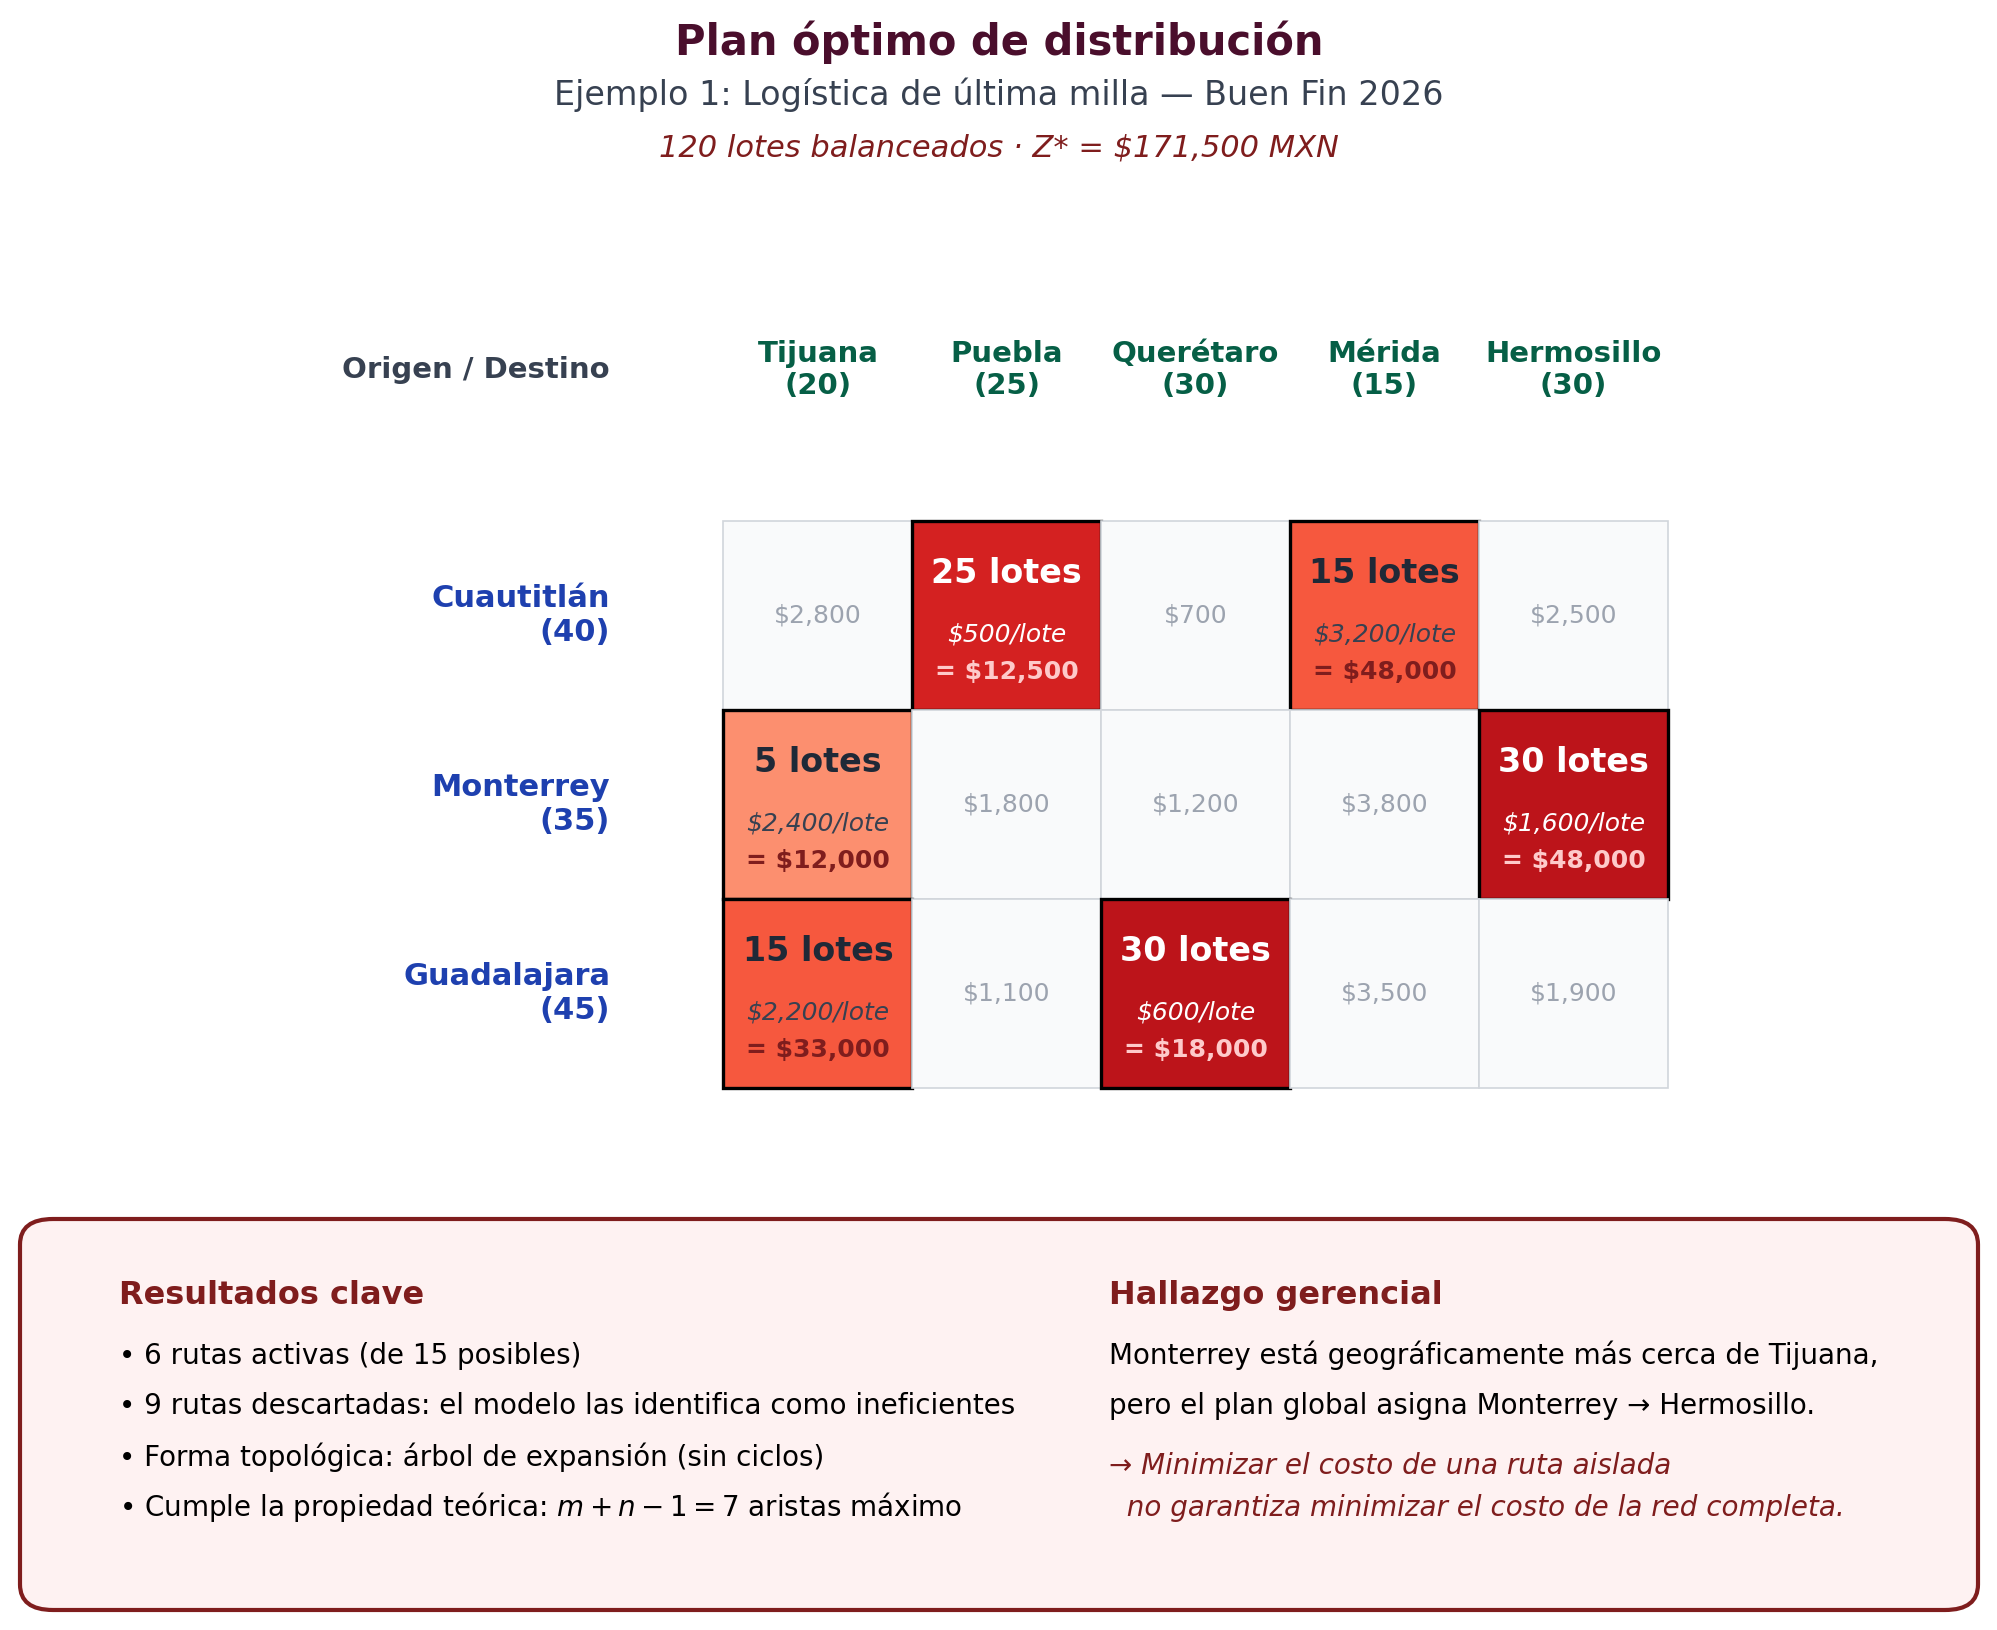
\includegraphics[width=0.78\textwidth]{img/fig6_matriz_ej1.png}
\caption{Plan óptimo de distribución del Ejemplo~1. Las celdas en rojo intenso corresponden a flujos altos; las celdas grises representan rutas no utilizadas. Los costos unitarios están expresados en MXN por lote. El subtotal de cada ruta activa aparece debajo del flujo en color rojo oscuro.}
\label{fig:matriz_ej1}
\end{figure*}

\begin{figure}[!h]
\centering
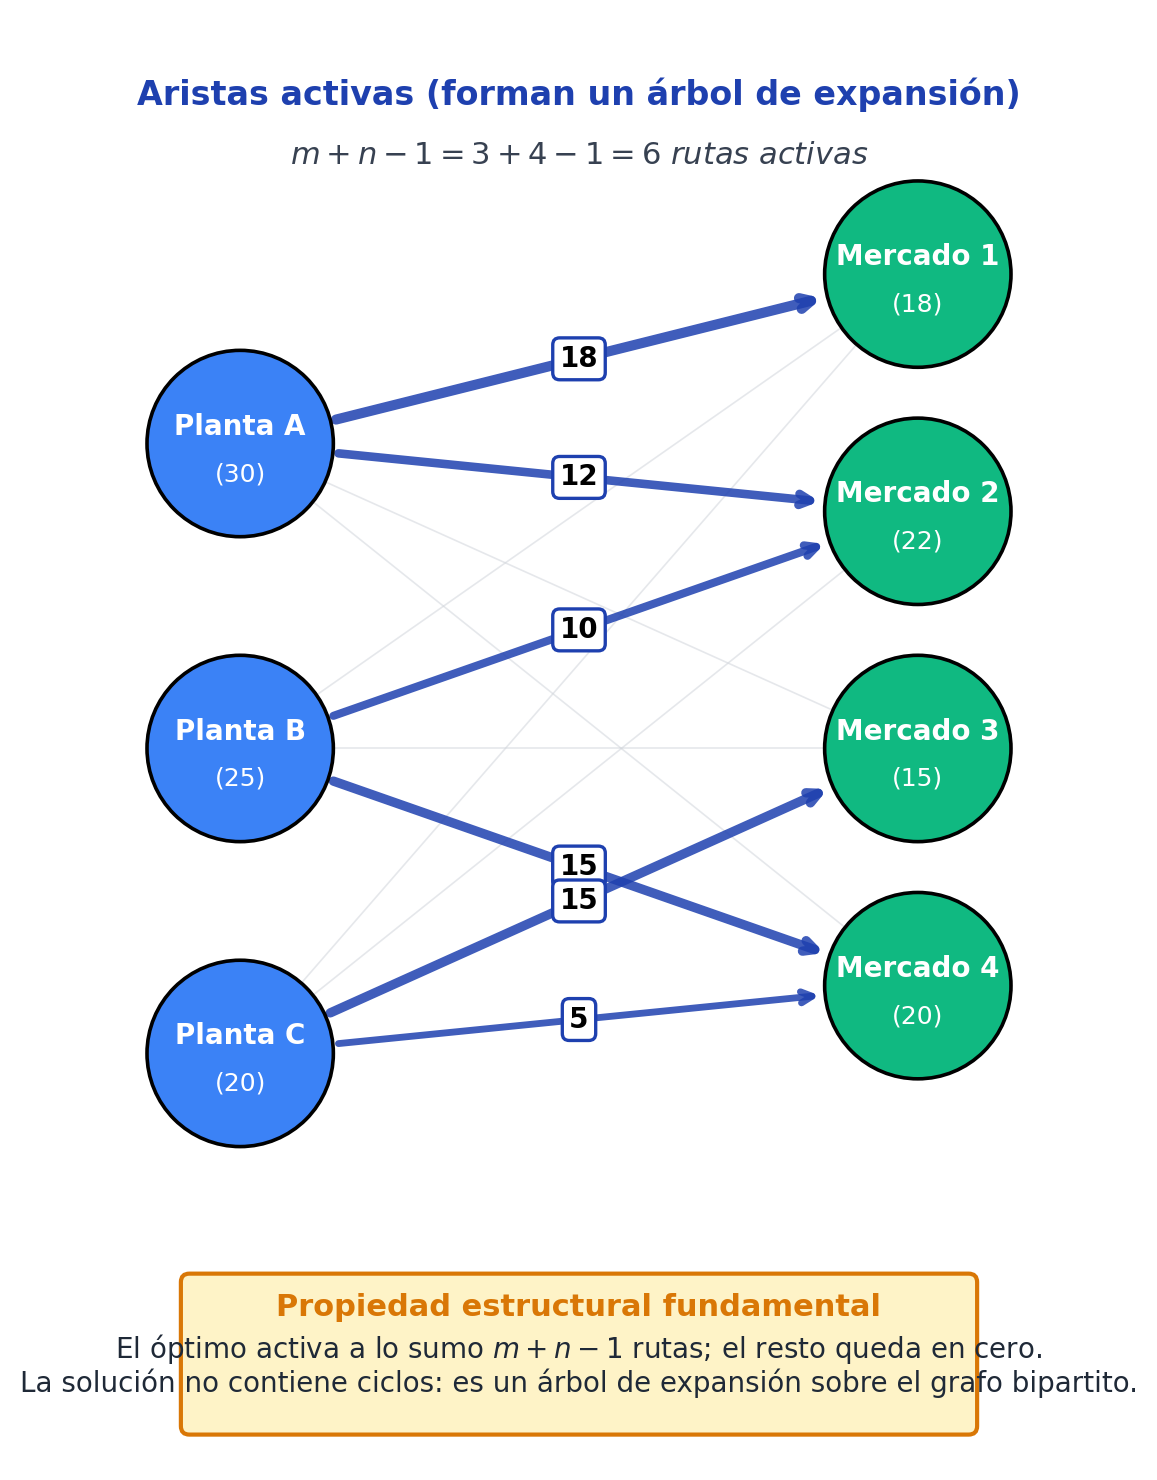
\includegraphics[width=\columnwidth]{img/fig7_arbol_expansion_ej1.png}
\caption{Árbol de expansión óptimo del Ejemplo~1: sólo 6 de las 15 rutas posibles aparecen en la solución, exactamente $m+n-1=7-1=6$ aristas (una menos que el máximo teórico, lo que se conoce como \emph{solución degenerada}). Las aristas se colorean según el origen y su grosor es proporcional al volumen transportado.}
\label{fig:arbol_expansion}
\end{figure}

\textbf{Análisis de las decisiones del modelo.} Los resultados ilustran cómo la optimización basada en datos puede contradecir la intuición geográfica. Monterrey está considerablemente más cerca de Tijuana que Guadalajara, y un planeador podría haber asignado intuitivamente todo el inventario de Monterrey para cubrir Tijuana. Sin embargo, el modelo global determina que la capacidad de Monterrey genera mayor rentabilidad si se destina a Hermosillo, dejando que Guadalajara ---con un costo unitario más bajo hacia Tijuana--- cubra el faltante. La conclusión gerencial es directa: minimizar el costo de una ruta aislada no garantiza minimizar el costo total de la red.

\subsubsection*{Consideraciones operativas adicionales}
El modelo entrega la solución de menor costo, pero la implementación real durante una temporada de alta demanda como el «Buen Fin» requiere evaluar también restricciones de tiempo. Por ejemplo, la ruta activa Cuautitlán $\to$ Mérida (aproximadamente 1{,}300~km) cumple con el criterio de costo mínimo terrestre, pero excede operativamente el umbral de 24~horas necesario para cumplir la promesa de entrega «Full» al día siguiente. Para iteraciones futuras del modelo se recomienda penalizar ese tipo de rutas largas mediante la técnica de la «$M$ grande»: asignar un costo artificialmente alto a las rutas que excedan el tiempo de tránsito permitido obliga al algoritmo a evitarlas salvo que sea estrictamente indispensable usarlas.

\subsubsection{Análisis dual: precios sombra}
Resolviendo el modelo con variables continuas (en lugar de enteras) para que el solver reporte las variables duales, se obtienen los precios sombra de la \textbf{Tabla~IV}. Cada precio sombra responde la pregunta: \emph{¿cuánto cambiaría el costo total si la oferta del origen $i$ (o la demanda del destino $j$) aumentara una unidad?}.

\begin{table}[!h]
\caption{Precios sombra del Ejemplo~1.}
\centering
\small
\begin{tabular}{l r}
\arrayrulecolor{infotec}\toprule
\rowcolor{infotec}\textcolor{white}{\textbf{Restricción}} & \textcolor{white}{\textbf{$\pi$ (MXN)}} \\
\midrule
Oferta Cuautitlán  & 500 \\
Oferta Monterrey   & 1,000 \\
Oferta Guadalajara & 800 \\
Demanda Tijuana    & 1,400 \\
Demanda Puebla     & 0 \\
Demanda Querétaro  & $-200$ \\
Demanda Mérida     & 2,700 \\
Demanda Hermosillo & 600 \\
\bottomrule
\end{tabular}
\arrayrulecolor{black}
\\
\raggedright\fontsize{6.5pt}{7.5pt}\selectfont Los valores reportados son los multiplicadores de las restricciones en el óptimo, obtenidos numéricamente por el solver CBC con una precisión de $10^{-6}$. Los signos pueden interpretarse directamente como los precios sombra duales $u_i$ (oferta) y $v_j$ (demanda).
\end{table}

El precio sombra más alto corresponde a la demanda de Mérida (\$2{,}700/lote): si la demanda en Mérida aumentara en un lote, el costo total subiría \$2{,}700, lo que refleja el costo elevado de las rutas hacia esa ciudad. Por el contrario, el precio sombra de Puebla es cero, lo que significa que pequeños incrementos en la demanda de Puebla no encarecen apreciablemente el plan: el sistema tiene holgura para absorberlos. Estos valores son informativos de cuello de botella en una negociación o expansión de la red.

\subsubsection{Escalabilidad del modelo}
El modelo desarrollado es flexible y se adapta a escenarios más complejos sin cambios estructurales mayores. Para sistemas \emph{desbalanceados} se introduce un nodo ficticio según convenga; para \emph{restricciones de capacidad} en una ruta específica (cuando una ruta no puede transportar más de cierto volumen) basta con añadir una cota superior $x_{ij} \leq U_{ij}$; para \emph{rutas prohibidas} se omite la variable o se le asigna un costo penalizado mediante la técnica de la «$M$~grande»; para problemas con \emph{nodos de transbordo}, la formulación se adapta al principio general de conservación de flujo (entradas menos salidas igual a demanda neta) y se convierte en un problema de flujo en redes. Estas extensiones se ilustran en el Ejemplo~2.

\subsection{Ejemplo 2: Distribución de agua en emergencia con restricciones complejas}

\subsubsection{Planteamiento del problema}
Se modela la distribución de agua potable desde dos plantas potabilizadoras hacia cinco comunidades durante una contingencia. Lo que diferencia este ejercicio del problema clásico son tres restricciones adicionales con justificación física concreta:

\begin{itemize}
\item \textbf{Ruta bloqueada:} la tubería de Planta~B hacia la Colonia San Nicolás (C3) sufrió daños y no puede usarse durante la contingencia.
\item \textbf{Capacidades máximas:} la tubería de Planta~A hacia Las Palmas (C4) soporta hasta 40~Ml/día, y la de Planta~B hacia Col. Progreso (C2) hasta 30~Ml/día.
\item \textbf{Prioridad hospitalaria:} el Hospital Regional (C1) debe recibir al menos 30~Ml/día provenientes de Planta~A, considerada la fuente más confiable por protocolo de emergencia.
\end{itemize}

La \textbf{Tabla~V} resume parámetros, costos de bombeo y restricciones del escenario.

\begin{table}[!h]
\caption{Costos, oferta, demanda y restricciones del Ejemplo~2 (MXN/Ml).}
\centering
\fontsize{7.5pt}{9pt}\selectfont
\begin{tabular}{l c c c c c c}
\arrayrulecolor{infotec}\toprule
\rowcolor{infotec}\textcolor{white}{\textbf{Origen}} & \textcolor{white}{\textbf{C1}} & \textcolor{white}{\textbf{C2}} & \textcolor{white}{\textbf{C3}} & \textcolor{white}{\textbf{C4}} & \textcolor{white}{\textbf{C5}} & \textcolor{white}{\textbf{Of.}} \\
\midrule
Planta~A & 12 & 18 & 14 & 20\textsuperscript{*} & 16 & 180 \\
Planta~B & 10 & 15\textsuperscript{*} & --- & 17 & 13 & 140 \\
\midrule
\textbf{Dem.} & 50 & 40 & 60 & 55 & 45 & 250 \\
\bottomrule
\end{tabular}
\arrayrulecolor{black}
\\[0.04in]
\fontsize{7pt}{8pt}\selectfont \emph{\textsuperscript{*}~con capacidad máx.\quad ---: ruta bloqueada}
\end{table}

Nótese que el problema es \textbf{desbalanceado}: la oferta total (320~Ml) supera la demanda total (250~Ml), por lo que sobrarán 70~Ml que no se asignarán a ninguna comunidad. Esto se modela usando restricciones de oferta como desigualdad ($\leq$) en lugar de igualdad.

\subsubsection{Formulación matemática}
Sea $x_{ij}$ la cantidad de megalitros enviados desde la planta $i$ a la comunidad $j$. El programa lineal completo es:

\begin{equation*}
\begin{aligned}
\text{Min}\; Z =\;& 12 x_{A,1} + 18 x_{A,2} + 14 x_{A,3} + 20 x_{A,4} + 16 x_{A,5}\\
                  & + 10 x_{B,1} + 15 x_{B,2} + 17 x_{B,4} + 13 x_{B,5}
\end{aligned}
\end{equation*}

Sujeto a:
\begin{itemize}
\item \textbf{Oferta:} $\sum_j x_{A,j} \leq 180$;\quad $\sum_j x_{B,j} \leq 140$.
\item \textbf{Demanda:} $x_{A,j} + x_{B,j} \geq b_j$ para cada comunidad $j$.
\item \textbf{Capacidades:} $x_{A,4} \leq 40$;\quad $x_{B,2} \leq 30$.
\item \textbf{Bloqueo:} $x_{B,3} = 0$.
\item \textbf{Prioridad:} $x_{A,1} \geq 30$.
\item \textbf{No negatividad:} $x_{ij} \geq 0$.
\end{itemize}

\subsubsection{Implementación en Python con PuLP}
El siguiente código implementa el modelo completo, lo resuelve y reporta los precios sombra de cada restricción:

\begin{lstlisting}
import pulp

# 1. Datos del problema
oferta  = [180, 140]
demanda = [50, 40, 60, 55, 45]
costo = [
  [12, 18, 14, 20, 16],   # Planta A
  [10, 15,  0, 17, 13],   # Planta B (0 = bloq)
]
plantas    = ["A", "B"]
comunidad  = ["C1_Hosp","C2_Progr","C3_SanNic",
              "C4_Palmas","C5_Carmen"]

# 2. Variables de decision
prob = pulp.LpProblem('Agua', pulp.LpMinimize)
x = [[pulp.LpVariable(f'x_{plantas[i]}_{j+1}',
                      lowBound=0)
      for j in range(5)] for i in range(2)]

# 3. Funcion objetivo (B->C3 bloqueada)
prob += pulp.lpSum(
    costo[i][j] * x[i][j]
    for i in range(2) for j in range(5)
    if not (i == 1 and j == 2))

# 4a. Restricciones de oferta
for i in range(2):
    prob += pulp.lpSum(x[i][j]
              for j in range(5)) <= oferta[i]

# 4b. Restricciones de demanda
for j in range(5):
    prob += pulp.lpSum(x[i][j]
              for i in range(2)) >= demanda[j]

# 4c. Restricciones especiales
prob += x[0][3] <= 40,  'Capacidad_A_C4'
prob += x[1][1] <= 30,  'Capacidad_B_C2'
prob += x[1][2] == 0,   'Bloqueo_B_C3'
prob += x[0][0] >= 30,  'Prioridad_Hosp_A'

# 5. Resolver
prob.solve(pulp.PULP_CBC_CMD(msg=0))
print(f"Z* = ${pulp.value(prob.objective):.0f}")
\end{lstlisting}

\subsubsection{Resultados}
El solver regresa el estado \emph{Optimal}: encontró un plan que satisface todas las restricciones simultáneamente. El costo mínimo diario es $\boldsymbol{Z^* = \$3{,}570 \text{~pesos/día}}$. La \textbf{Figura~\ref{fig:matriz_ej2}} muestra el plan óptimo en formato de matriz, con los flujos, costos unitarios y subtotales por celda.

\begin{figure*}[!t]
\centering
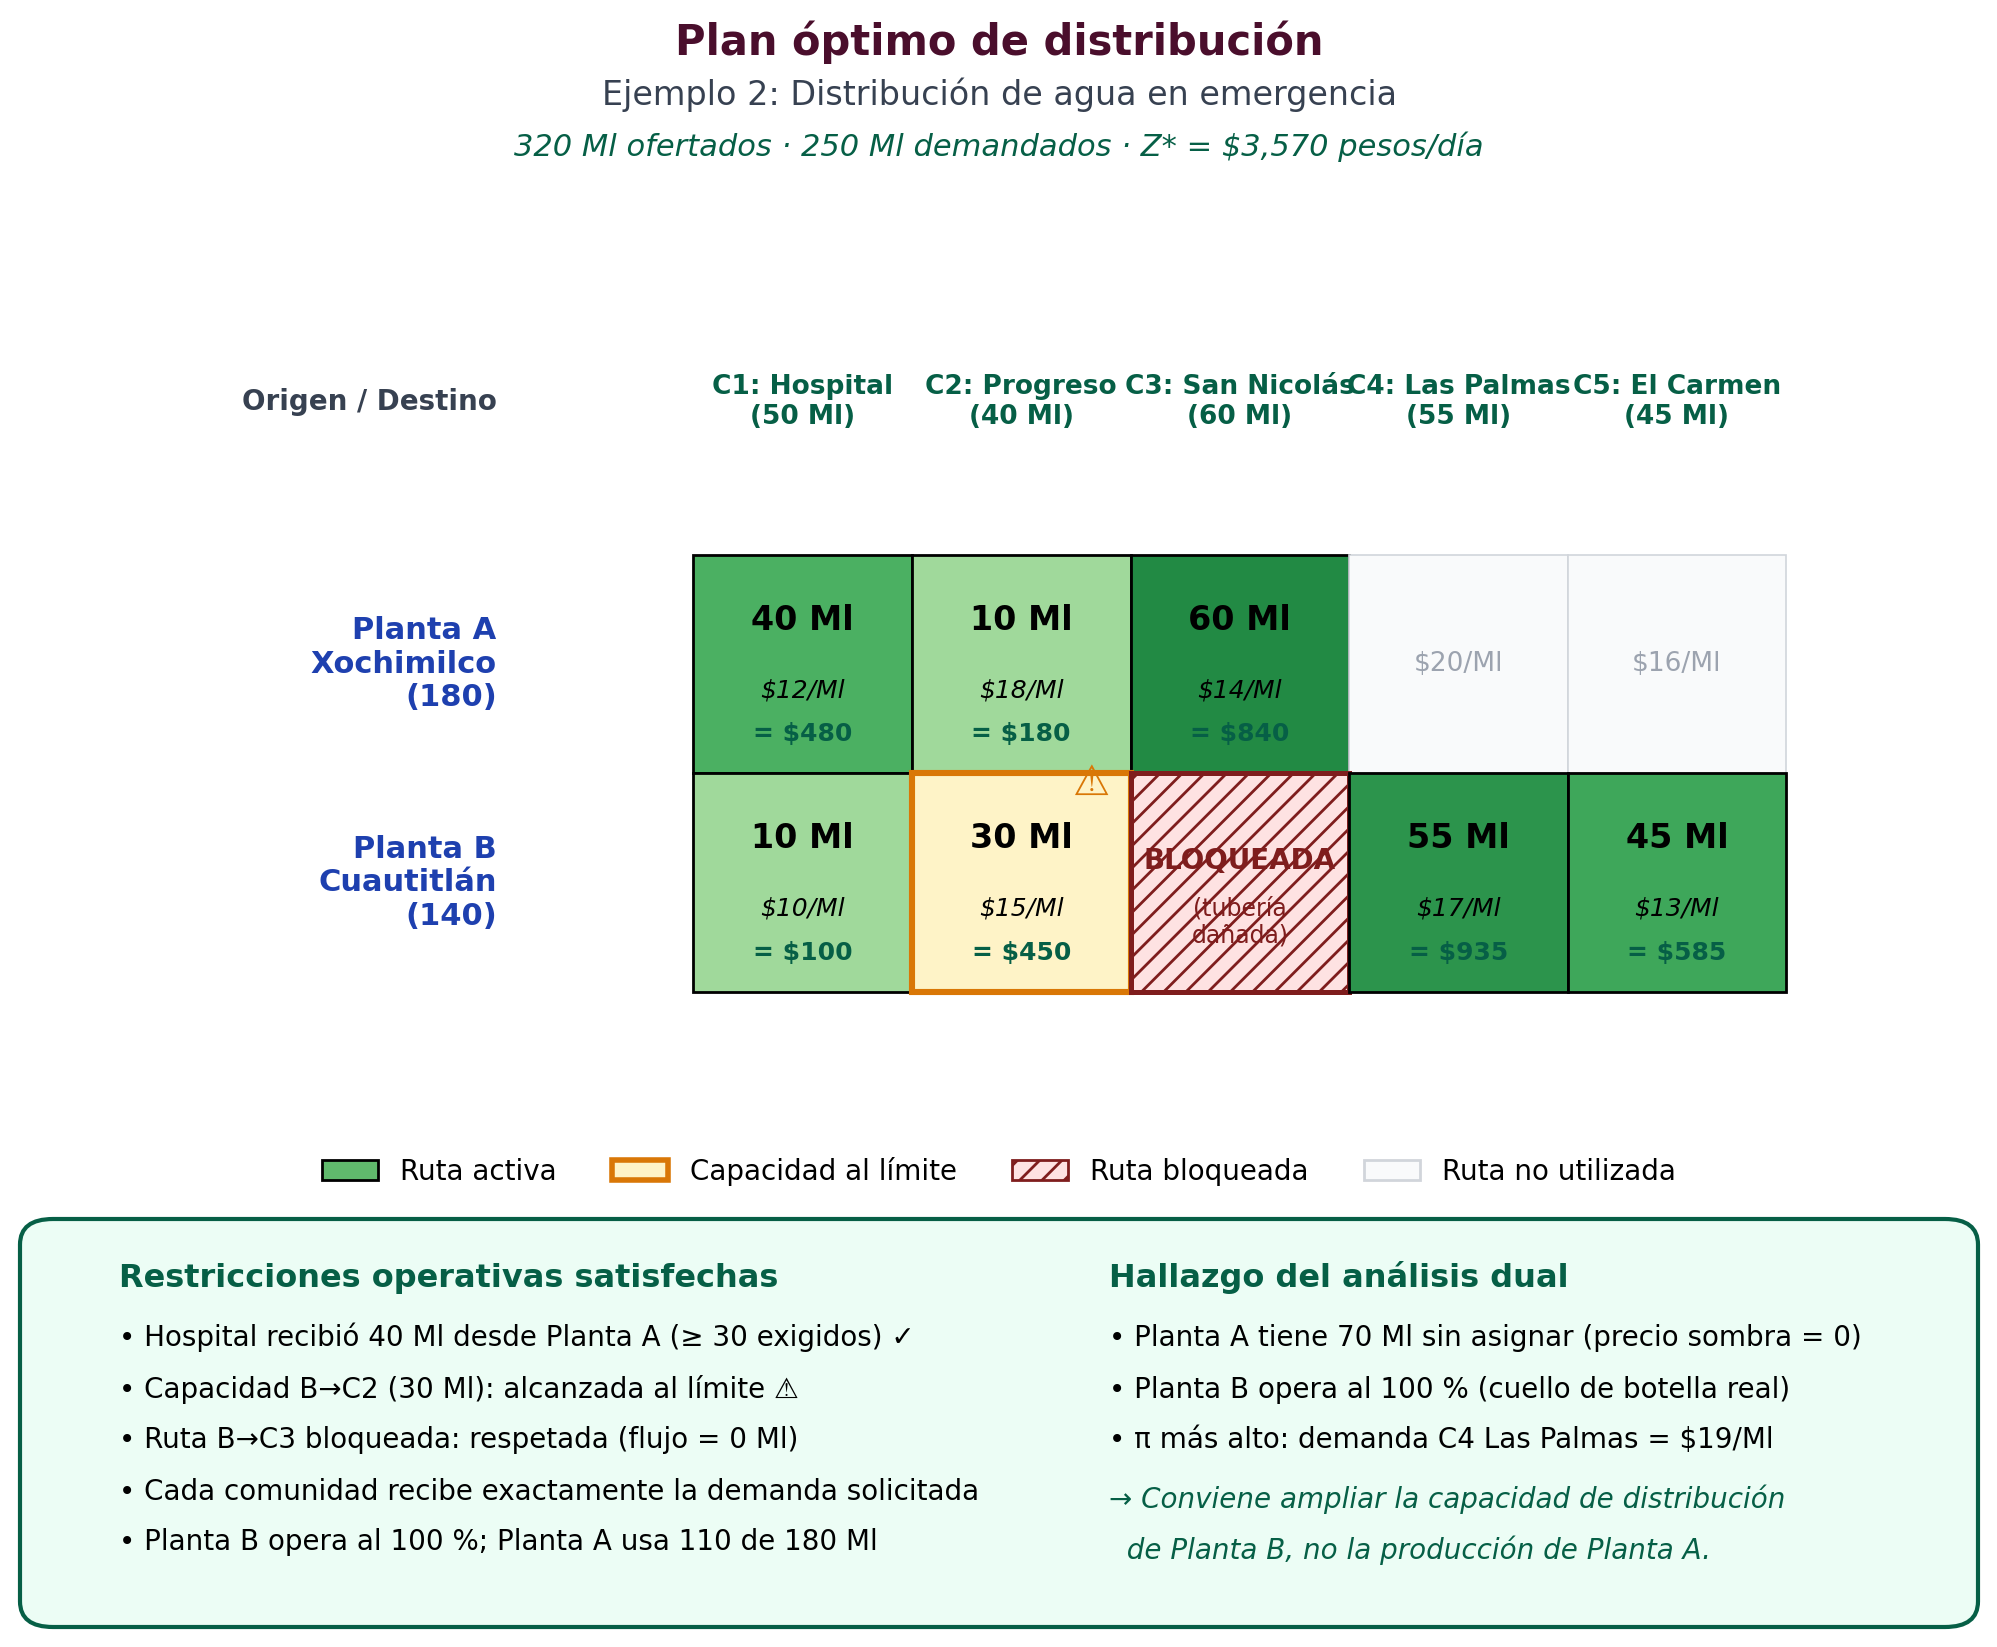
\includegraphics[width=0.85\textwidth]{img/fig8_matriz_ej2.png}
\caption{Plan óptimo del Ejemplo~2 con restricciones complejas. La intensidad del verde es proporcional al volumen asignado; la celda en amarillo señala una capacidad alcanzada y la celda con franjas rojas representa la ruta bloqueada.}
\label{fig:matriz_ej2}
\end{figure*}

El detalle numérico se presenta en la \textbf{Tabla~VI}.

\begin{table}[!h]
\caption{Plan óptimo de distribución de agua --- Ejemplo~2.}
\centering
\fontsize{7.5pt}{9pt}\selectfont
\begin{tabular}{l l r r r}
\arrayrulecolor{infotec}\toprule
\rowcolor{infotec}\textcolor{white}{\textbf{Origen}} & \textcolor{white}{\textbf{Destino}} & \textcolor{white}{\textbf{Flujo}} & \textcolor{white}{\textbf{Costo}} & \textcolor{white}{\textbf{Subtotal}} \\
\midrule
Planta~A & C1 Hospital     & 40.0 & \$12 & \$480 \\
Planta~A & C2 Progreso     & 10.0 & \$18 & \$180 \\
Planta~A & C3 San Nicolás  & 60.0 & \$14 & \$840 \\
Planta~B & C1 Hospital     & 10.0 & \$10 & \$100 \\
Planta~B & C2 Progreso     & 30.0 & \$15 & \$450 \\
Planta~B & C4 Las Palmas   & 55.0 & \$17 & \$935 \\
Planta~B & C5 El Carmen    & 45.0 & \$13 & \$585 \\
\midrule
\multicolumn{2}{l}{\textbf{Total}} & \textbf{250.0} & --- & \textbf{\$3{,}570} \\
\bottomrule
\end{tabular}
\arrayrulecolor{black}
\end{table}

\textbf{Verificación de las restricciones.} Antes de interpretar los resultados, conviene verificar que el plan respeta todas las restricciones. La oferta de Planta~A se utilizó parcialmente (110 de 180~Ml; sobran 70). Planta~B operó al 100\,\% de su capacidad. Cada comunidad recibió exactamente la demanda solicitada. La ruta bloqueada Planta~B$\to$C3 quedó en cero, como se exigía. La capacidad de Planta~A$\to$C4 (40~Ml) no se alcanzó (de hecho, esa ruta no se usó). La capacidad de Planta~B$\to$C2 (30~Ml) sí se alcanzó exactamente. Y la prioridad hospitalaria se cumplió: el Hospital recibió 40~Ml desde Planta~A ---diez por encima del mínimo exigido--- más 10~Ml desde Planta~B.

\subsubsection{Análisis de precios sombra}
Un precio sombra responde la pregunta: \emph{¿cuánto cambiaría el costo total si esta restricción se relajara una unidad?}. La \textbf{Tabla~VII} resume los valores obtenidos.

\begin{table}[!h]
\caption{Precios sombra del Ejemplo~2 e interpretación.}
\centering
\fontsize{7pt}{8.5pt}\selectfont
\begin{tabular}{p{1.6cm} c p{4cm}}
\arrayrulecolor{infotec}\toprule
\rowcolor{infotec}\textcolor{white}{\textbf{Restricción}} & \textcolor{white}{\textbf{$\pi$}} & \textcolor{white}{\textbf{Interpretación}} \\
\midrule
Demanda C1 Hospital     & \$12 & Si la demanda del hospital aumenta 1~Ml, el costo sube \$12. \\
Demanda C2 Progreso     & \$18 & Costo marginal por demanda más alto del lado del transportista. \\
Demanda C3 San Nicolás  & \$14 & Sólo Planta~A puede abastecer esta zona; el recurso es escaso. \\
Demanda C4 Las Palmas   & \textbf{\$19} & Mayor precio sombra: cuello de botella crítico. \\
Demanda C5 El Carmen    & \$15 & Se abastece exclusivamente desde Planta~B. \\
Capacidad B$\to$C2 (30~Ml) & $-\$1$ & El signo negativo indica que ampliar 1~Ml ahorraría apenas \$1/día (el solver reporta $\pi$ negativo para cotas superiores activas). \\
Oferta Planta~A          & \$0 & Producir más agua en Planta~A no reduce el costo: ya sobra. \\
\bottomrule
\end{tabular}
\arrayrulecolor{black}
\end{table}

Tres hallazgos destacan. \textbf{Primero}, el precio sombra más alto corresponde a la demanda de Las Palmas (\$19/Ml): si esa comunidad necesitara un megalitro adicional, el costo total subiría \$19/día. Es el cuello de botella más caro del sistema. \textbf{Segundo}, la restricción de capacidad B$\to$C2 tiene precio sombra de apenas un peso, así que ampliar esa tubería ahorraría muy poco y no justifica una inversión grande. \textbf{Tercero}, el sobrante de Planta~A (70~Ml/día sin asignar) tiene precio sombra cero: producir más agua ahí no aporta nada al sistema, porque el verdadero cuello de botella está en la capacidad de distribución de Planta~B, que ya opera al 100\,\%. La \textbf{Figura~\ref{fig:sensibilidad_ej2}} permite visualizar esta jerarquía de precios sombra de un vistazo: la longitud de cada barra indica el impacto marginal de relajar la restricción correspondiente. Una recomendación gerencial directa surge del análisis: en lugar de aumentar la producción de Planta~A, conviene invertir en ampliar la capacidad de distribución de Planta~B.

\begin{figure*}[!t]
\centering
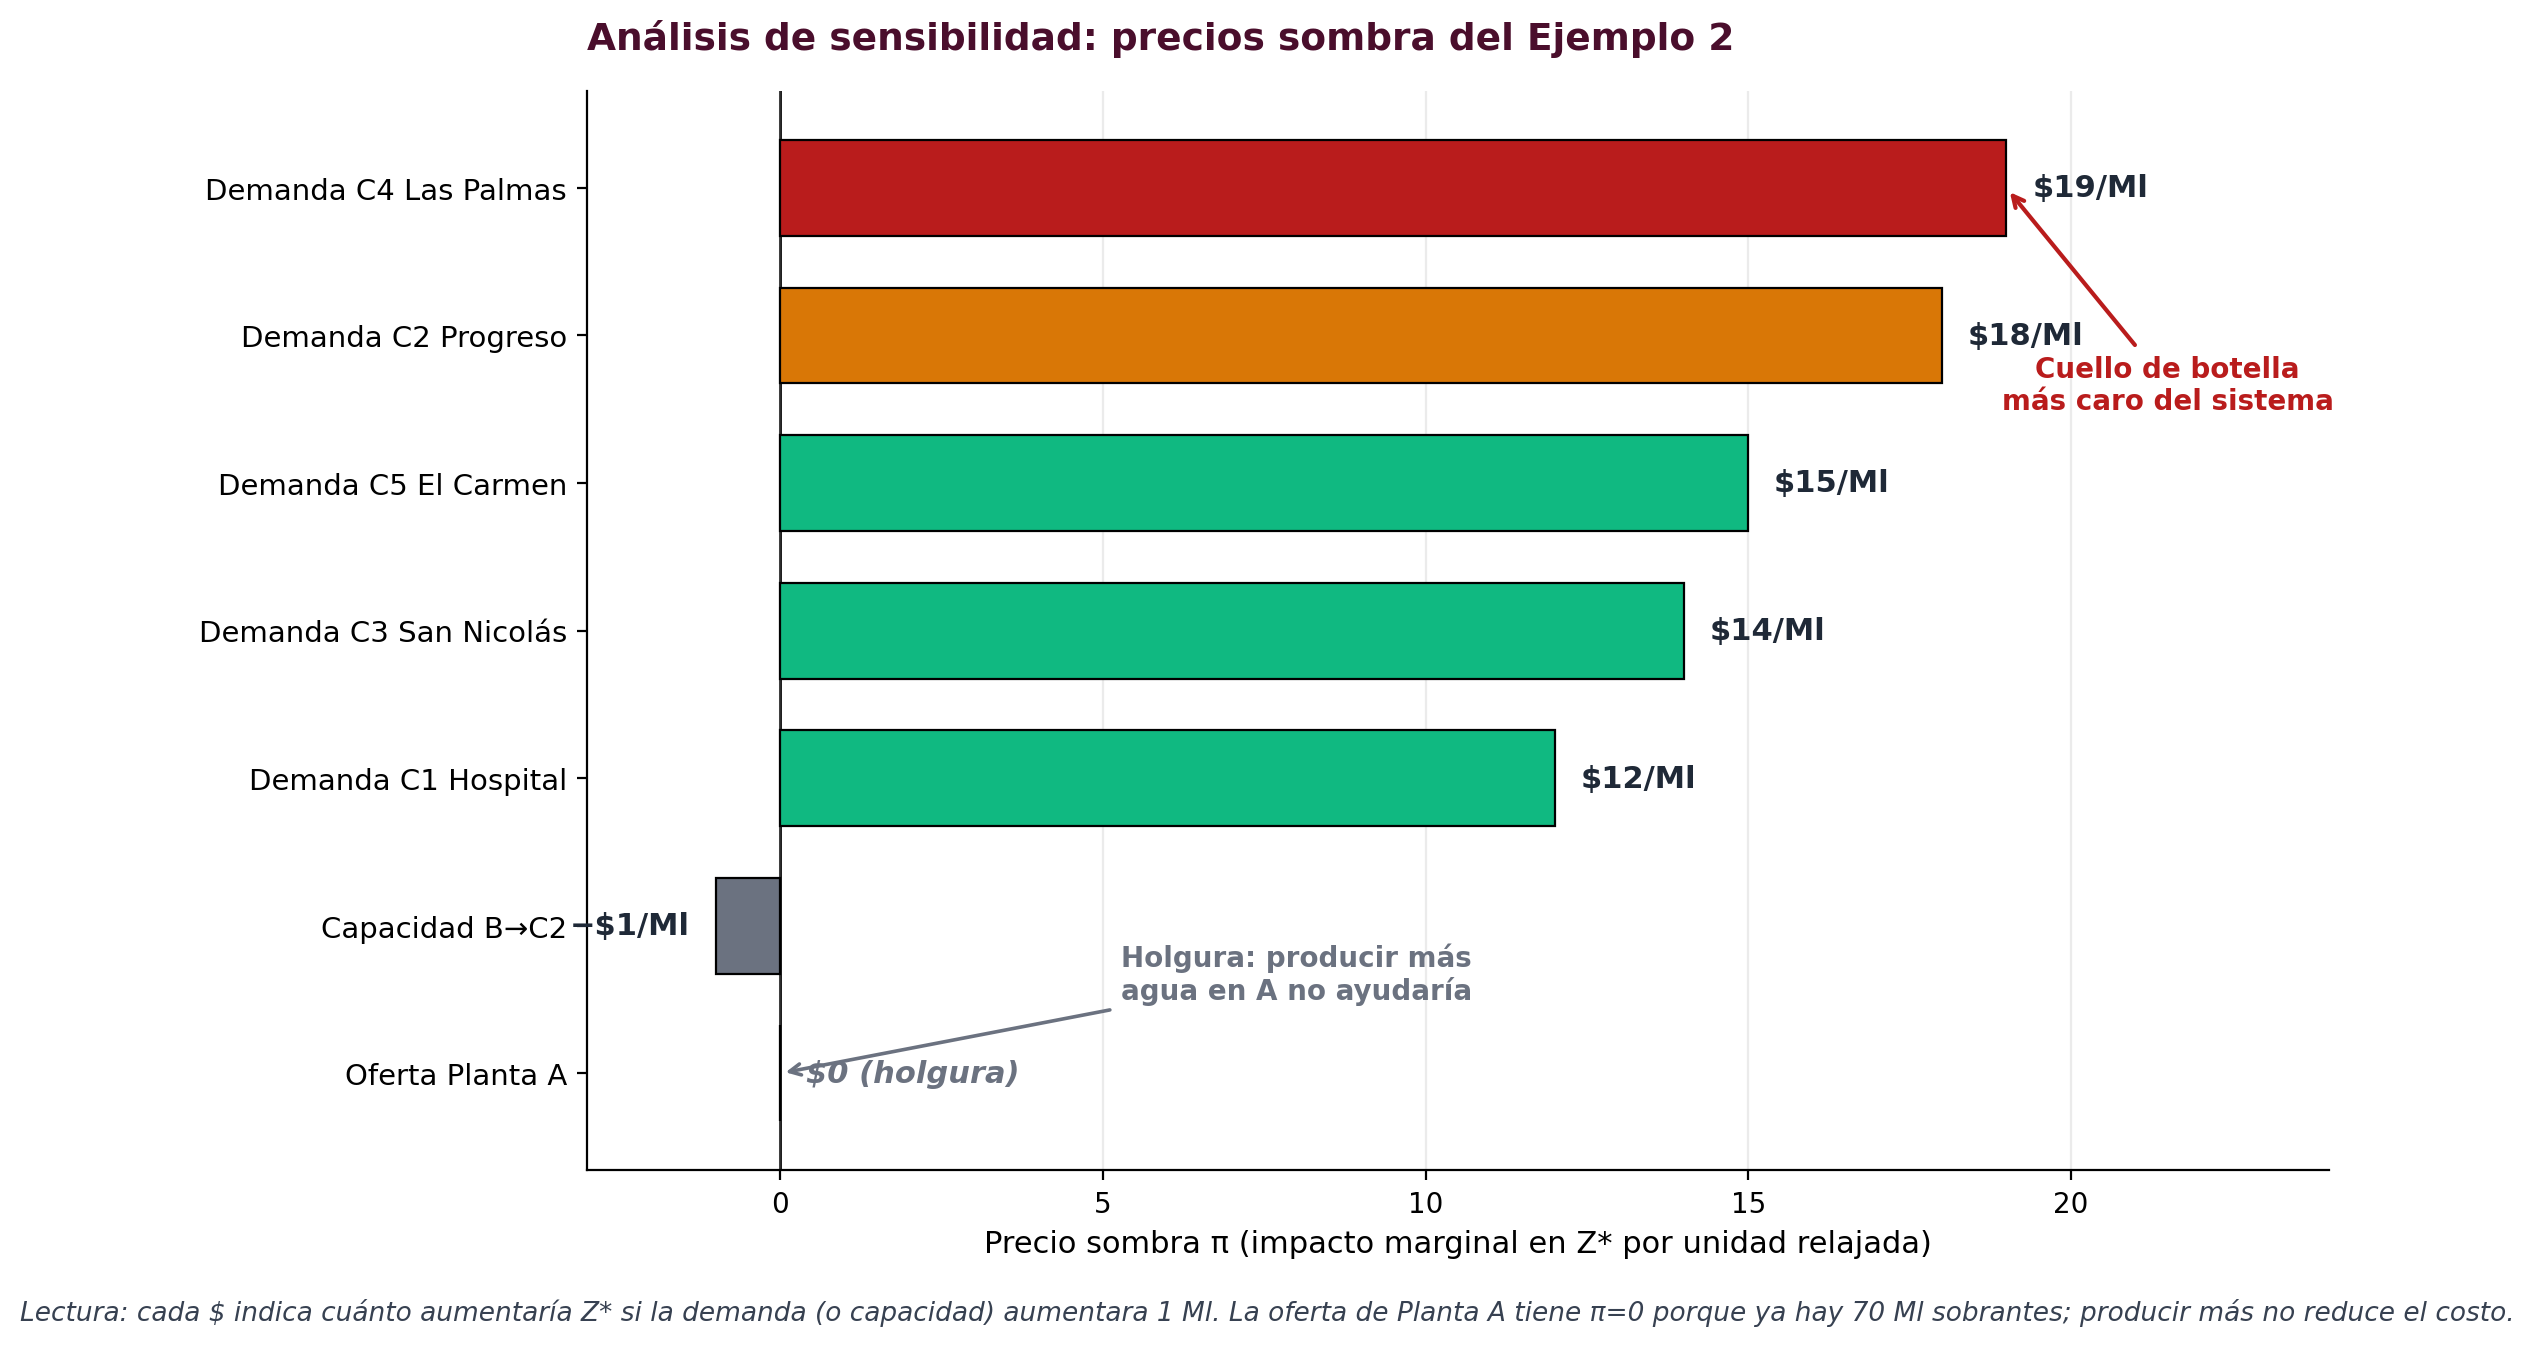
\includegraphics[width=0.9\textwidth]{img/fig9_sensibilidad_ej2.png}
\caption{Análisis de sensibilidad del Ejemplo~2: precios sombra ordenados por magnitud. La barra roja superior identifica el cuello de botella crítico del sistema (demanda de Las Palmas, \$19/Ml). Las dos restricciones inferiores con $\pi \leq 0$ indican holgura: la capacidad B$\to$C2 con valor $-\$1$ por convención del solver, y la oferta de Planta~A con $\pi = 0$ (los 70~Ml sobrantes no aportan al costo). La gráfica permite priorizar inversiones de capacidad de un vistazo.}
\label{fig:sensibilidad_ej2}
\end{figure*}

% ============================================================
%  5. APLICACIONES PRÁCTICAS
% ============================================================
\section{Aplicaciones Prácticas}

El modelo del transporte funciona en cualquier escenario donde existan puntos con excedente de algo (fábricas, plantas, almacenes) y puntos con necesidad de ese algo (tiendas, comunidades, subestaciones), y se busque mover entre ellos al menor costo posible. Las áreas siguientes son las aplicaciones más consolidadas.

\subsection{Logística y cadena de suministro}
El uso más natural del modelo es asignar qué almacén surte a qué tienda minimizando los costos de flete. FEMSA Comercio, por ejemplo, opera más de 20{,}000 tiendas OXXO abastecidas desde múltiples centros de distribución regionales; la decisión de qué CEDIS surte a qué tienda, considerando capacidades vehiculares y ventanas de entrega, es exactamente el problema del transporte. A esta escala, una solución bien resuelta puede traducirse en ahorros logísticos millonarios al año.

\subsection{Distribución de recursos en emergencias}
El modelo se usa para repartir agua, medicamentos o alimentos al menor costo respetando prioridades y rutas disponibles ---exactamente como en el Ejemplo~2. El Centro Nacional de Prevención de Desastres (CENAPRED) en México emplea modelos análogos para preposicionar suministros antes de temporadas de huracanes o sismos: se colocan inventarios en bodegas regionales de modo que, si ocurre el desastre, el costo de distribuirlos hacia las zonas afectadas sea mínimo.

\subsection{Redes eléctricas}
El modelo de transporte se usa en su forma extendida (flujo en redes) para decidir cuánta energía genera cada planta y hacia qué subestación se envía, minimizando las pérdidas en transmisión. El Centro Nacional de Control de Energía (CENACE) emplea modelos de este tipo para despachar energía en el Sistema Eléctrico Nacional. Las líneas de transmisión tienen capacidades máximas que se modelan como las restricciones de capacidad del Ejemplo~2.

\subsection{Movilidad urbana}
El \emph{modelo gravitacional de distribución de viajes}~[4] usa la misma estructura: zonas residenciales como orígenes, zonas de trabajo o comercio como destinos, y un costo (tiempo o distancia) que se minimiza. Se aplica al diseño de rutas del Metro de la Ciudad de México y a la planeación de corredores de transporte público.

\subsection{Limitaciones del modelo}
Conviene reconocer dónde el modelo clásico se queda corto:

\begin{itemize}
\item \textbf{No representa rutas con escalas.} Sólo modela origen y destino directo. Si hay nodos intermedios de transbordo, se requiere el problema de flujo en redes.
\item \textbf{Asume costos lineales.} Si existe un costo fijo por «abrir» una ruta ---independientemente de cuánto se transporte---, hace falta programación entera mixta.
\item \textbf{Asume un solo tomador de decisiones.} Cuando transportista, embarcador y regulador tienen objetivos opuestos, se debe recurrir a teoría de juegos o programación bi-nivel~[6].
\end{itemize}

% ============================================================
%  6. CONCLUSIONES
% ============================================================
\section{Conclusiones}

El Problema del Transporte es un punto de encuentro raro en investigación de operaciones: combina una teoría matemática profunda con una utilidad práctica inmediata. Las cuatro conclusiones siguientes intentan capturar esa doble naturaleza tomando como referencia tanto el desarrollo teórico de la Sección~3 como los dos ejemplos numéricos de la Sección~4.

\textbf{Primero, la dualidad no es un artificio matemático: es una lectura económica del problema.} La Sección~3.2 mostró que detrás de cada restricción primal (oferta o demanda) hay una variable dual con interpretación de precio sombra, y que la condición de holgura complementaria $x_{ij}^*(c_{ij}-u_i-v_j)=0$ reproduce exactamente el principio de equilibrio espacial de precios formulado por Cournot en 1838: el precio en un mercado de destino no puede exceder al del origen más el costo de transporte. Esto conecta el modelo lineal con un razonamiento microeconómico clásico sobre arbitraje. El Ejemplo~2 confirmó la utilidad práctica de esa lectura: los precios sombra de la Tabla~VII permitieron identificar que ampliar la capacidad de distribución de Planta~B sería estratégicamente más valioso que aumentar la producción de Planta~A, una recomendación que el plan óptimo por sí solo no entrega. Es decir, el plan dice \emph{qué hacer}, los precios sombra dicen \emph{dónde duele más una unidad de cambio}, y la teoría de dualidad explica \emph{por qué} ambas vistas son consistentes entre sí.

\textbf{Segundo, la topología del problema es la clave de su tratabilidad.} La representación como grafo bipartito desarrollada en la Sección~3.3 no es un recurso pedagógico, sino una propiedad estructural: el rango del sistema es $m+n-1$, la solución óptima forma un árbol de expansión sin ciclos y la matriz de coeficientes es totalmente unimodular. Estas tres propiedades juntas explican que un solver pueda resolver instancias con miles de variables en milisegundos. En el Ejemplo~1 se confirmó empíricamente que de las 15 rutas posibles sólo 6 quedaron activas en el óptimo, formando exactamente un árbol de expansión. Reconocer esta estructura permite, además, diseñar algoritmos especializados (esquina noroeste, costo mínimo, Vogel, multiplicadores) que aprovechan la geometría del problema para resolverlo más rápido que el simplex general.

\textbf{Tercero, las restricciones operativas reales no rompen el modelo: lo enriquecen.} Una crítica habitual al problema clásico es que su formulación parece demasiado simple para situaciones operativas. El Ejemplo~2 mostró lo contrario: agregar una ruta físicamente bloqueada, dos capacidades máximas en tuberías y una prioridad hospitalaria fue cuestión de añadir cuatro líneas de código en \texttt{PuLP}, sin alterar la estructura general del modelo. El sistema sigue siendo lineal, sigue siendo resoluble en milisegundos, y los precios sombra siguen teniendo interpretación económica. La lección operativa es directa: una vez que se domina la formulación primal-dual y su contraparte computacional, modelar nuevos escenarios deja de ser un problema de matemáticas y se convierte en un problema de explicitar correctamente las reglas del negocio. Esta facilidad es lo que convierte al modelo en una herramienta interactiva de planeación, no sólo en un ejercicio académico.

\textbf{Cuarto, todo modelo tiene fronteras y reconocerlas es parte del oficio.} El equilibrio primal-dual del modelo clásico supone un único tomador de decisiones, costos lineales y un grafo estrictamente bipartito. Cuando alguno de estos supuestos falla ---costos fijos por abrir una ruta, nodos intermedios de transbordo, transportista y embarcador con intereses en conflicto--- el modelo necesita extenderse hacia programación entera mixta, flujo de costo mínimo en redes generales o programación bi-nivel. El propio caso del Ejemplo~1 anticipó este límite: una ruta puede ser óptima en costo (Cuautitlán~$\to$ Mérida) y simultáneamente inviable por restricciones de tiempo de tránsito, lo que obliga a penalizarla con la técnica de la $M$~grande o a reformular el problema. Reconocer cuándo el modelo clásico es suficiente y cuándo conviene escalarlo es tan importante como saber resolverlo.

En conjunto, estas cuatro lecciones explican por qué ochenta años después de su formulación por Hitchcock el Problema del Transporte sigue siendo vigente: combina rigor matemático (dualidad, unimodularidad, árboles de expansión), eficiencia computacional (solvers especializados que lo resuelven en milisegundos) e interpretabilidad gerencial directa (precios sombra que apuntan a cuellos de botella reales). Esa triple cualidad ---rigor, eficiencia e interpretabilidad--- es difícil de encontrar junta en otros modelos de optimización, y es lo que mantiene al Problema del Transporte como una de las herramientas básicas de la investigación de operaciones moderna.

% ============================================================
%  7. REFERENCIAS
% ============================================================
\section{Referencias Bibliográficas}

\small
\begin{enumerate}[leftmargin=1.2em,itemsep=0.4ex]
\item Moreno Q., E. (2005). El problema del Transporte: Una interpretación del dual. \emph{NOTAS del Instituto Mexicano del Transporte}, núm.~93. Secretaría de Comunicaciones y Transportes, México.
\item Taha, H.~A. (2017). \emph{Operations Research: An Introduction} (10.\textsuperscript{a}~ed.). Pearson Education Limited.
\item Bazaraa, M.~S., Jarvis, J.~J. y Sherali, H.~D. (2009). \emph{Linear Programming and Network Flows} (4.\textsuperscript{a}~ed.). John Wiley \& Sons.
\item Ortúzar, J.~D. y Willumsen, L.~G. (1994). \emph{Modelling Transport} (2.\textsuperscript{a}~ed.). John Wiley \& Sons.
\item Cournot, A. (1838). \emph{Researches into the Mathematical Principles of the Theory of Wealth} (traducción al inglés de N.~T.~Bacon, 1927). The Macmillan Co., Nueva York.
\item Moreno, E. (2004). \emph{Planner--User Interactions in Road Freight Transport: A Modelling Approach with a Case Study from Mexico} (Tesis doctoral). Institute for Transport Studies, University of Leeds, Reino Unido.
\item Dantzig, G.~B. (1963). \emph{Linear Programming and Extensions}. Princeton University Press.
\item Hitchcock, F.~L. (1941). The Distribution of a Product from Several Sources to Numerous Localities. \emph{Journal of Mathematics and Physics}, 20(1--4), 224--230.
\item Kantorovich, L.~V. (1939). \emph{Mathematical Methods of Organizing and Planning Production}. Leningrad State University.
\item Koopmans, T.~C. (1949). Optimum Utilization of the Transportation System. \emph{Econometrica}, 17 (Supplement), 136--146.
\item Kuhn, H.~W. (1955). The Hungarian Method for the Assignment Problem. \emph{Naval Research Logistics Quarterly}, 2(1--2), 83--97.
\item Ford, L.~R. y Fulkerson, D.~R. (1956). Maximal Flow through a Network. \emph{Canadian Journal of Mathematics}, 8, 399--404.
\item Schrijver, A. (1986). \emph{Theory of Linear and Integer Programming}. John Wiley \& Sons.
\item Ahuja, R.~K., Magnanti, T.~L. y Orlin, J.~B. (1993). \emph{Network Flows: Theory, Algorithms, and Applications}. Prentice Hall.
\item Mitchell, S., O'Sullivan, M. y Dunning, I. (2011). \emph{PuLP: A Linear Programming Toolkit for Python}. The University of Auckland.
\item López Ruiz, F. y Arana Landín, G. (2002). La dualidad en el problema de transporte. \emph{VI Congreso de Ingeniería de Organización}, Vigo, España.
\item COIN-OR Foundation. (2024). \emph{PuLP: A linear programming toolkit for Python}. \url{https://coin-or.github.io/pulp/}
\item Diestel, R. (2017). \emph{Graph Theory} (5.\textsuperscript{a}~ed.). Springer.
\item COIN-OR Foundation. (2024). \emph{A Transportation Problem --- PuLP case study}. \url{https://coin-or.github.io/pulp/CaseStudies/a_transportation_problem.html}
\item The SciPy Community. (2024). \emph{scipy.optimize.linprog --- SciPy v1.17.0 Manual}.
\item NEOS Guide. (2022). \emph{Linear Programming}. National Science Foundation, University of Wisconsin--Madison.
\item Bridgelall, R. (2022). \emph{Tutorial and practice in linear programming: Optimization problems in supply chain and transport logistics}. North Dakota State University. \url{https://arxiv.org/pdf/2211.07345}
\item Virtanen, P. et al. (2020). SciPy~1.0: Fundamental Algorithms for Scientific Computing in Python. \emph{Nature Methods}, 17, 261--272.
\end{enumerate}

% =====================================================
%  ANEXO A — Notebook ejecutable
% =====================================================
\onecolumn
\newpage
\thispagestyle{empty}

\vspace*{2in}
\begin{center}
{\sffamily\bfseries\color{infotec}\fontsize{24pt}{28pt}\selectfont
Anexo A\par}
\vspace{0.3in}
{\sffamily\bfseries\fontsize{18pt}{22pt}\selectfont
Notebook ejecutable\par}
\vspace{0.2in}
{\sffamily\itshape\large
Reproducción computacional íntegra de los modelos del reporte\par}
\vspace{0.5in}
\begin{minipage}{4.5in}
\centering\small
Las páginas siguientes corresponden a la ejecución completa del notebook
\texttt{transporte\_equipo5.ipynb} en Google Colab. Incluye los modelos
teórico (Sección~3.3.1), del Ejemplo~1 (Sección~4.1) y del Ejemplo~2
(Sección~4.2), con todas las salidas intermedias, los precios sombra y
las visualizaciones del grafo bipartito generadas por NetworkX.\\[0.15in]
El notebook fuente está disponible en el repositorio del equipo.
\end{minipage}
\end{center}

% Inclusión del PDF del notebook ejecutado.
\IfFileExists{notebook_ejecutado.pdf}{%
  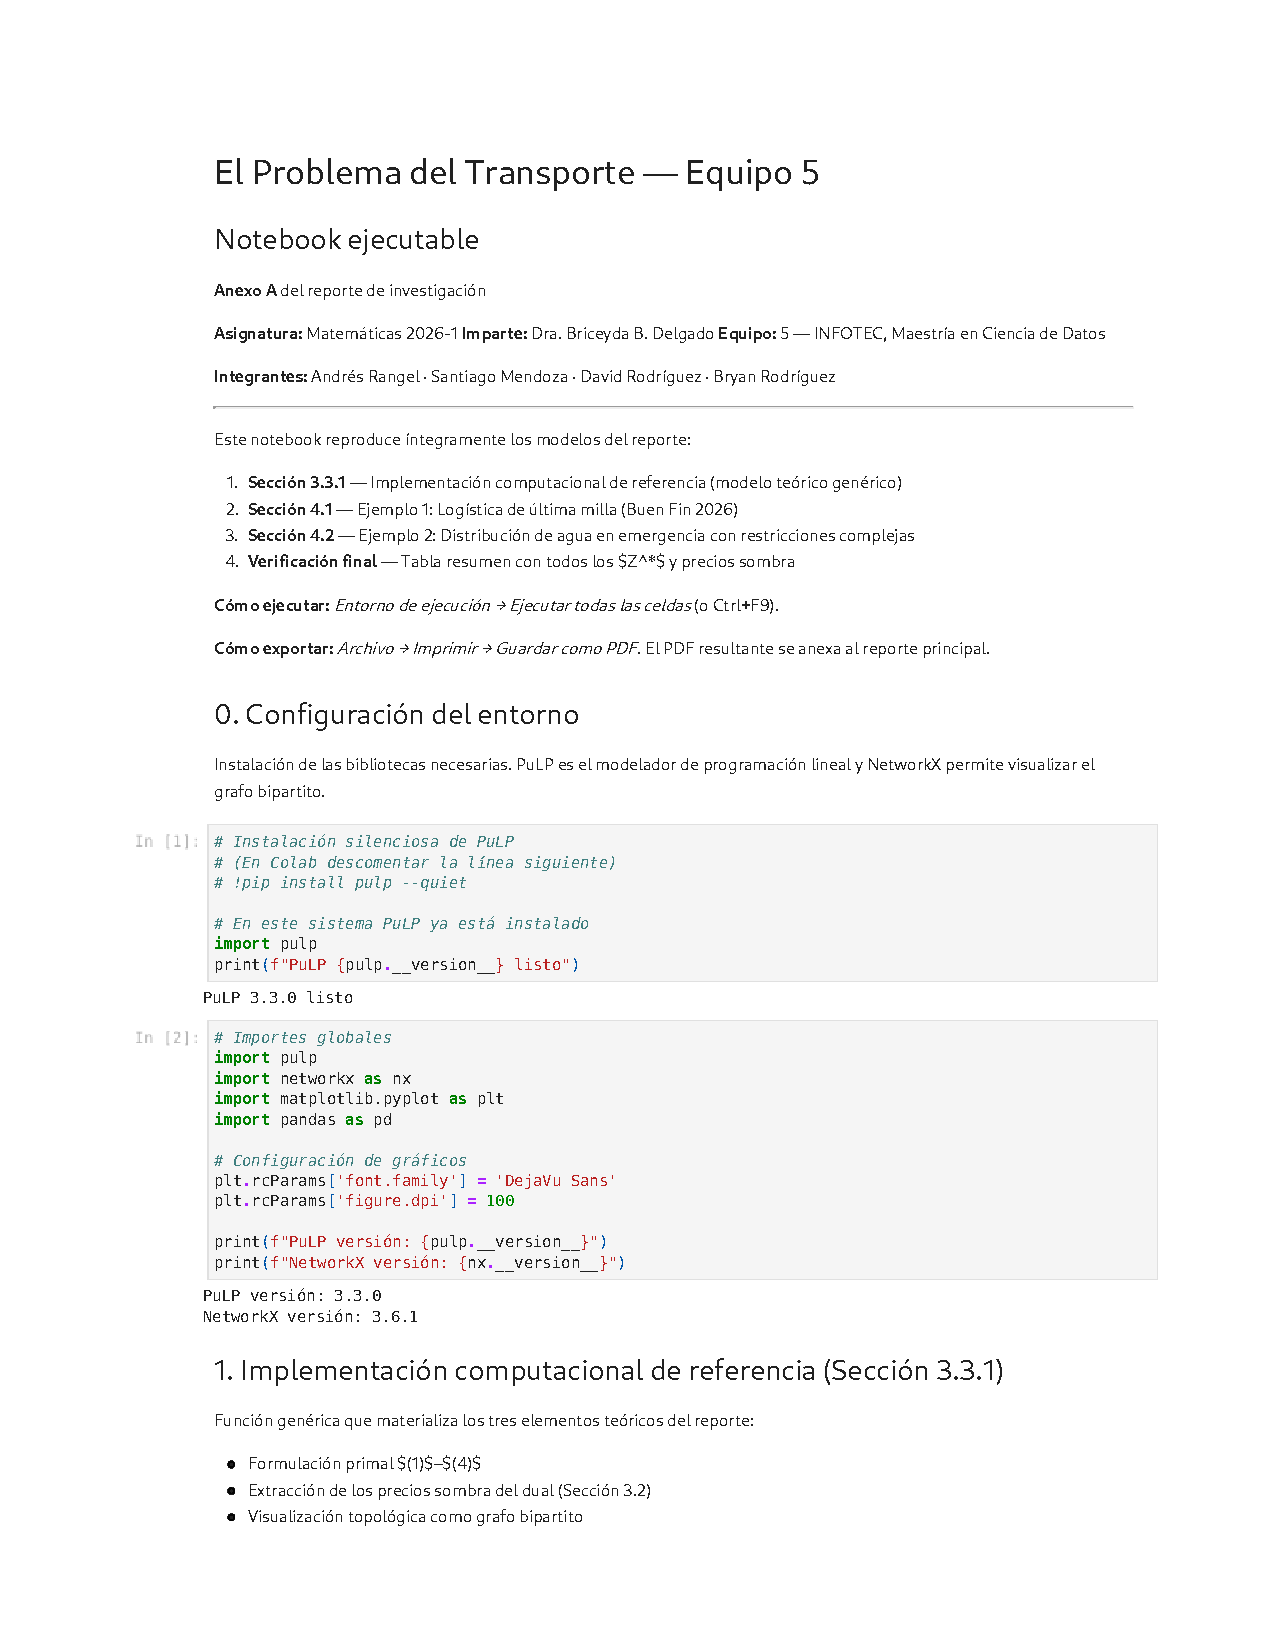
\includepdf[pages=-,pagecommand={\thispagestyle{plain}},
              fitpaper=true, frame=false]{notebook_ejecutado.pdf}%
}{%
  \begin{center}
  \vspace*{1in}
  \fbox{\begin{minipage}{0.7\textwidth}
  \centering\small
  \textbf{Nota para el editor del documento:}\\[0.1in]
  Para incluir aquí el notebook ejecutado, exporta el archivo
  \texttt{transporte\_equipo5.ipynb} como PDF desde Colab
  (\textit{Archivo $\to$ Imprimir $\to$ Guardar como PDF}) y guárdalo
  como \texttt{notebook\_ejecutado.pdf} en la misma carpeta que
  \texttt{reporte.tex}. Recompila el documento.
  \end{minipage}}
  \end{center}
}

\end{document}